\documentclass[12pt, a4paper]{report}

% Encoding and fonts
\usepackage[utf8]{inputenc}
\usepackage[T1]{fontenc}
\usepackage{mathptmx}   % Times New Roman (text + math)

% Math
\usepackage{amsmath}
\usepackage{amsfonts}
\usepackage{amssymb}

% Tables and figures
\usepackage{booktabs}
\usepackage{threeparttable}
\usepackage{graphicx}
\usepackage{float}

% Layout
\usepackage[margin=2.5cm]{geometry}
\usepackage{setspace}
\onehalfspacing

% Lists
\usepackage{enumitem}

% Abstract
\usepackage{abstract}

% Bibliography
\usepackage[round,authoryear,semicolon]{natbib}

% Cross-referencing and links (load last)
\usepackage[hidelinks]{hyperref}

% ------------------------------------------------------------------
% Front matter
% ------------------------------------------------------------------

\begin{document}

\begin{titlepage}
\centering
\vspace*{2cm}
{\fontsize{14}{18}\selectfont
\textbf{Do LLMs Shape the Diffusion of New Software?}\\[6pt]
\textbf{Training Cutoffs and Adoption Dynamics in the Python Ecosystem}
}\\[2cm]
{\fontsize{14}{18}\selectfont
Roland Tuboly\\[6pt]
Social Data Science MSc, 1st year\\[2cm]
Supervisor: Johannes Wachs
}\\[2cm]
{\fontsize{14}{18}\selectfont
Budapesti Corvinus Egyetem\\[6pt]
2026
}
\vfill
\end{titlepage}

\begin{abstract}
\noindent
Large language models are trained on fixed snapshots of public knowledge, creating a boundary between tools the model can recommend and tools it cannot. This paper asks whether that boundary shapes the diffusion of newly released open-source software. I study the Python ecosystem around the September 2021 GPT-3.5/GPT-4 training cutoff, using PyPI download counts for 527,361 packages and GitHub import data for 28,243 matched libraries.

The identification strategy is a sharp regression discontinuity design (RDD) with a nine-week donut exclusion for libraries whose training-data inclusion is ambiguous. The main causal estimate comes from a difference-in-discontinuities (Diff-in-RDD) specification that differences the 2021 discontinuity against placebo discontinuities at the same calendar position in 2018--2020. Inference uses bias-corrected local linear estimation with a fixed bandwidth of $h = 13$ weeks and cluster-robust standard errors.

Three findings emerge. First, post-cutoff libraries suffer a significant diffusion penalty once LLMs reach mass adoption: the Diff-in-RDD estimate is $-12.8$ log points for libraries that achieved at least 500 downloads in their first 26 weeks ($p = 0.008$). Post-cutoff libraries were more successful before ChatGPT, making the reversal conservative. Second, the penalty is roughly twice as large in GitHub code imports ($26.8$ log points) as in PyPI downloads ($13.1$ log points), consistent with LLM-steered code generation as the channel. Third, the gap was absent in all placebo years and emerged only after November 2022. As of January 2026, no catch-up is observed.

The results provide evidence that LLM training cutoffs function as a structural barrier to entry, a ``Knowledge Wall,'' that redirects adoption toward already-known tools. Limitations include imperfect proxy measurement, an underpowered mechanism test, and local identification.

\vspace{0.5cm}
\noindent \textbf{Keywords:} Regression Discontinuity Design, Large Language Models, Training Data Cutoff, Software Adoption, Python Ecosystem, Knowledge Diffusion, Open Source Software.
\end{abstract}
\newpage

\pagenumbering{roman}
\tableofcontents
\newpage
\listoftables
\newpage
\listoffigures
\newpage

\pagenumbering{arabic}

% ------------------------------------------------------------------
% Chapter 1
% ------------------------------------------------------------------
\chapter{Introduction}\label{ch:intro}

\section{The Problem}\label{sec:intro-problem}
Large language models (LLMs) have become a standard interface through which software developers discover libraries, generate code, and diagnose errors. GitHub Copilot, ChatGPT, and their successors are now embedded in development workflows across the skill distribution, from novice programmers to professional engineers at large technology firms. As of 2024, over half of professional developers report regular use of AI coding assistants \citep{stackoverflow2024survey}, and the share of code in public repositories with detectable AI-generation signatures has grown continuously since the public release of ChatGPT in November 2022.

This transformation raises a structural question: if LLMs function as an intermediary between developers and the software library ecosystem, the temporal boundary of their training data creates a systematic asymmetry in developer access to knowledge. Libraries released before a cutoff are visible; those after are not. This paper provides an empirical answer for the Python package ecosystem.

\section{The Mechanism}\label{sec:intro-mechanism}
The proposed mechanism operates through a specific property of pretrained language models: their parametric knowledge is fixed at training time. A model trained on data through September 2021 has no intrinsic knowledge of a library first released in November 2021, regardless of that library's quality, functionality, or subsequent adoption. When a developer asks such a model to recommend a library for a given task, or when the model generates code to accomplish a task, the post-cutoff library is not part of the candidate set. The pre-cutoff library, even an older or less capable one, is.

This asymmetry is not hypothetical. The GPT-3.5 and GPT-4 model families, which powered the majority of AI coding assistant usage in 2022--2024, share a documented training data cutoff of September 27, 2021 (OpenAI, 2023). A Python library released on September 26, 2021 was a candidate for inclusion in these models' knowledge; a library released on September 28, 2021 was not. If LLM recommendations shape adoption, this discrete boundary should produce a detectable discontinuity in the diffusion trajectories of libraries released just before versus just after the cutoff.

The causal chain is therefore: \textbf{training cutoff $\rightarrow$ differential knowledge representation $\rightarrow$ differential LLM recommendation frequency $\rightarrow$ differential developer adoption}. Each link is plausible; the empirical question is whether the chain is strong enough to produce measurable population-level effects in observational data.

\section{The Research Gap}\label{sec:intro-gap}
The consequences of AI deployment for collective knowledge and creative diversity have attracted recent theoretical interest. \citet{doshi2024generative} demonstrate in a controlled experiment that generative AI improves the average quality of individual creative output while simultaneously reducing the diversity of outputs across participants. Individuals assisted by AI converge toward similar high-quality solutions, compressing collective exploration. The implication is that AI systems which improve individual productivity may reduce the aggregate variety of ideas, products, and approaches that a community generates.

The software ecosystem offers a tractable empirical setting in which to test whether an analogous logic operates for tool adoption. If LLMs steer developers toward pre-cutoff libraries, the collective variety of tools in active use may narrow over time, not because post-cutoff libraries are inferior, but because they are unknown to the intermediary through which developers now routinely access the ecosystem. This would represent a \textit{Knowledge Wall}: a concentration mechanism that is invisible to any individual developer but operates at the aggregate level to shape the distribution of tool adoption.

The empirical literature on technology diffusion and platform economics has documented how recommendation systems, network effects, and algorithmic curation influence product adoption, but has not yet addressed the role of LLM training boundaries as a specific mechanism. The software ecosystem literature documents factors shaping library survival and adoption, but predates the mass deployment of AI coding assistants. This paper sits at the intersection of these two bodies of work, contributing an empirically identified estimate of a mechanism specific to the current moment.

\section{Research Setting}\label{sec:intro-setting}
The Python Package Index (PyPI) provides an unusually well-suited setting for this investigation. Python is the dominant language for data science, machine learning, and scientific computing, precisely the domains in which AI-assisted coding is most prevalent. PyPI records weekly download counts for every registered package, enabling the construction of library-level diffusion curves that begin at the week of first observed adoption. GitHub complements this with implementation-level evidence: a panel of weekly import counts per library, with an additional layer of commit-level AI scoring that indicates the probability that each importing commit was generated with LLM assistance.

The combination of these sources allows the question to be asked at two levels. First, does the training cutoff affect general developer adoption, as measured by PyPI downloads? Second, does it specifically affect AI-mediated code generation, as measured by the subset of GitHub imports attributable to AI-assisted commits? If the effect is larger in the latter, this is evidence that the channel runs through LLM-generated code rather than general attention or discoverability. A documented, precisely dated knowledge cutoff (September 27, 2021) enables clean identification through a Regression Discontinuity Design.

\section{Research Questions and Hypotheses}\label{sec:intro-hypotheses}
The central question is: \textit{Do Python libraries released shortly before the GPT-3.5/GPT-4 training cutoff diffuse more widely in the AI era than those released shortly after?}

\begin{description}[style=multiline, leftmargin=3em]
    \item[H1:] Pre-cutoff libraries exhibit greater post-AI diffusion than post-cutoff libraries.
    \item[H2:] The discontinuity is larger in GitHub imports than in PyPI downloads.
    \item[H3:] The gap emerged only after the mass deployment of ChatGPT (Nov 2022).
    \item[H4:] Placebo cutoffs in 2018–2020 do not produce comparable discontinuities.
\end{description}

\section{Design Overview}\label{sec:intro-design}
The primary strategy is a \textbf{Difference-in-Discontinuities (Diff-in-RDD)} design. The 2021 cohort is compared against 2018--2020 placebo cohorts to control for seasonal patterns. An asymmetric donut exclusion handles data pipeline lags, and success tiers are defined based on pre-ChatGPT performance to avoid selection bias.

\section{Preview of Findings}\label{sec:intro-preview}
The evidence supports the existence of a Knowledge Wall. After controlling for historical seasonal patterns through the Diff-in-RDD design, libraries released just after the September 2021 training cutoff show a significantly lower post-AI adoption trajectory than libraries released just before it. The suppression is concentrated among libraries that demonstrated pre-ChatGPT quality (those that achieved meaningful early adoption without AI assistance) rather than being driven by low-quality noise at the boundary. It is substantially larger in GitHub implementation than in PyPI downloads, consistent with the LLM code generation channel. And it was dormant before November 2022, activating only when ChatGPT provided a mass interface through which the training boundary became consequential for developer behavior.

A separate test shows that post-cutoff libraries are less likely to ever achieve a meaningful adoption threshold, implying that the Knowledge Wall operates at entry, not only at subsequent growth stages.

\section{Contribution}\label{sec:intro-contribution}
This paper makes three contributions. First, it provides, to the best of the author's knowledge, the first quasi-experimental estimate of the causal effect of LLM training data boundaries on the diffusion of new software packages. The identification strategy exploits a documented institutional feature (the precision-dated GPT-3.5/GPT-4 training cutoff) to generate a clean discontinuity in expected knowledge representation. Second, it introduces a two-outcome research design that distinguishes general developer adoption (PyPI) from implementation-level usage (GitHub), enabling the identification of a channel effect not available from download data alone. Third, it provides empirical grounding for the theoretical concern, articulated by \citet{doshi2024generative} in the context of creative output, that AI systems which improve individual productivity may simultaneously narrow collective adoption diversity, here concretized in the specific mechanism of training data boundaries.

\section{Paper Structure}\label{sec:intro-structure}
Chapter~\ref{ch:lit} reviews the relevant literature across four bodies of work: AI and collective diversity, algorithmic monoculture, technology diffusion theory, and LLM knowledge boundaries. Chapter~\ref{ch:data} describes the data sources and sample construction. Chapter~\ref{ch:methods} formalizes the empirical design. Chapter~\ref{ch:results} presents the results. Chapter~\ref{ch:discussion} interprets findings and discusses limitations. A final chapter concludes.

% ------------------------------------------------------------------
% Chapter 2
% ------------------------------------------------------------------
\chapter{Literature Review}\label{ch:lit}

This chapter situates the paper within four bodies of scholarship. Section~\ref{sec:lit-creativity} covers the emerging literature on AI and collective diversity. Section~\ref{sec:lit-monoculture} reviews research on algorithmic monoculture and platform concentration. Section~\ref{sec:lit-diffusion} develops the theoretical context from technology diffusion and innovation ecology. Section~\ref{sec:lit-productivity} surveys empirical work on LLMs in economic activity. Section~\ref{sec:lit-boundaries} covers technical work on LLM knowledge boundaries and their practical limits. Section~\ref{sec:lit-contribution} states precisely what this paper adds.

\section{AI, Creativity, and Collective Diversity}\label{sec:lit-creativity}

The central theoretical concern motivating this paper is that tools which improve individual productivity may simultaneously narrow the collective variety of outputs they help produce. The most direct empirical grounding for this concern is \citet{doshi2024generative}, who conduct a preregistered online experiment in which participants wrote short stories with or without access to a generative AI system. Access to AI increased average story quality, consistent with individual productivity gains. The same access, however, caused the distribution of outputs to contract: stories written with AI assistance were more similar to one another than stories written by humans alone. The authors interpret this as a social dilemma. Each individual is better off with AI assistance; yet the aggregate range of novel content produced is narrower. The mechanism is convergence: AI suggestions push participants toward similar high-quality solutions, compressing the exploratory variety that human writers would otherwise generate.

The analogy to software adoption is structural, not empirical. Doshi and Hauser study creative text; this paper examines tool selection. The logic, however, is the same. When developers query an LLM for library recommendations, the model draws on parametric knowledge to suggest options. If many developers query the same model, they receive correlated suggestions concentrated on the libraries best represented in training data. The collective effect is a narrowing of the active tool set, not because post-cutoff libraries are worse, but because the information intermediary cannot consider them. Doshi and Hauser (2024) serve as a motivation and a structural analogy for this paper; they are not directly comparable empirical evidence.

Related experimental evidence strengthens the micro-level plausibility of this mechanism. \citet{anderson2024homogenization} examine creative ideation in an experiment where participants used either ChatGPT or an alternative creativity support tool. Users of ChatGPT generated more detailed ideas but less semantically distinct ones than users of the alternative tool. The homogenization was group-level rather than individual: different users received similar suggestions from the same model, converging on similar ideas even when working independently. This group-level convergence is precisely the mechanism that would, if replicated in the domain of library discovery, produce the population-level adoption pattern this paper identifies. \citet{wu2025generative} document a closely related phenomenon at the model output level, introducing the concept of generative monoculture: LLM outputs exhibit narrower diversity than the distribution of the underlying training data, a property they trace to alignment via reinforcement learning from human feedback rather than to corpus composition. This finding implies that even updating training data would not eliminate the concentration pressure, since the alignment process itself promotes convergence toward modal outputs.

\citet{raghavan2024competition} provides a theoretical counterpoint using a game-theoretic model, showing that competition among AI providers selects for diverse outputs at equilibrium, potentially mitigating monoculture. The empirical implication is that homogenization pressure may dissipate as model variety increases. The competitive equilibrium result applies, however, to markets with genuinely differentiated providers. It does not address the case studied in this paper, where multiple dominant models (GPT-3.5, GPT-4, Copilot) shared a common training cutoff during the period of mass deployment and therefore a common knowledge boundary. Competition may moderate monoculture in outputs; it does not eliminate a shared temporal constraint in training data.

\section{Algorithmic Monoculture and Platform Concentration}\label{sec:lit-monoculture}

The broader literature on algorithmic monoculture addresses the systemic risks that arise when shared decision systems are deployed at scale. \citet{kleinberg2021algorithmic} formalize the core argument in a probabilistic framework: when multiple decision-makers adopt the same algorithm, the correlation in their decisions reduces collective decision quality even if the algorithm is individually optimal, because correlated errors cannot be diversified away. Applied to library discovery, when many developers query the same LLM, their exploration of the ecosystem is correlated, concentrating adoption on the same subset of pre-cutoff tools and reducing the effective diversity of the solutions they produce.

\citet{bommasani2022picking} extend this framework to foundation models specifically. Testing whether shared model components homogenize outcomes across decision-makers in vision and language tasks, they find that sharing training data reliably increases outcome homogenization at the individual level, with effects that exceed group-level averages. Their result is directly relevant to the mechanism proposed in this paper: when developers share the same base model, the correlation in library suggestions is an empirical prediction of their framework, not a speculative concern.

The broader infrastructure risks of foundation model concentration are catalogued in \citet{bommasani2022foundation}, a comprehensive technical report covering the societal implications of models trained on broad corpora and adapted to downstream tasks at scale. The report identifies homogenization as a first-order risk: concentrated model infrastructure creates correlated failure modes across applications. The Knowledge Wall described in this paper is a specific instance of this general risk, operating through the temporal dimension of training data rather than through the breadth of model deployment.

\section{Technology Diffusion and Innovation Ecology}\label{sec:lit-diffusion}

The study of how new technologies spread through populations has a long lineage in economics and sociology. \citet{bass1969new} established the foundational diffusion model, decomposing adoption into two components: innovators, who adopt independently of social influence, and imitators, who are influenced by the number of prior adopters. In the contemporary software ecosystem, LLMs have entered the adoption process as a new type of information intermediary mediating the imitation channel. For a library to reach imitators through LLM-mediated discovery, it must first be represented in the model's parametric knowledge. Libraries outside the model's training corpus are excluded from the LLM recommendation channel, effectively reducing their access to a large share of the imitator population. The Knowledge Wall is a structural modification to the Bass imitation process, blocking a specific route through which new adopters would otherwise learn about a library.

\citet{rogers2003diffusion} characterized adopter categories from innovators through laggards and identified observability as a key attribute accelerating adoption: potential adopters are more likely to adopt a technology they can see in use. Observability is directly constrained by the Knowledge Wall. A library that the dominant LLM cannot recommend is less likely to appear in LLM-generated code, reducing its observability among developers who rely on AI-assisted workflows. Rogers's framework implies that reduced observability has first-order effects on adoption rates, particularly in the early majority phase where social proof begins to compound.

The general-purpose technology (GPT) framework of \citet{bresnahan1995general} characterizes transformative technologies by pervasiveness, ongoing improvement, and innovational complementarities, meaning that the technology stimulates R\&D and innovation in downstream sectors. \citet{eloundou2024gpts} confirm that LLMs satisfy these criteria. The Bresnahan and Trajtenberg framework also implies a specific failure mode: when a GPT's capabilities are temporally bounded, its innovational complementarities become path-dependent on the historical state of the complementary input space. Post-cutoff libraries are excluded from the LLM's complementary network at the point of mass deployment, concentrating the GPT's complementarity benefits on the pre-cutoff tool set.

\citet{weitzman1998recombinant} proposes that economic growth proceeds through combinatorial recombination of existing ideas, with the pace of innovation determined in part by the variety of components available for recombination. The Knowledge Wall restricts this process by narrowing the menu of components that the dominant discovery mechanism can present. If developers encounter only pre-cutoff libraries through LLM-mediated search, the combinatorial space available for software development converges over time toward the pre-cutoff universe. \citet{arthur2009nature} extends the same logic to technological evolution, arguing that new technologies are assembled from existing ones and that the available toolkit determines what combinations are feasible. A frozen LLM knowledge base acts as a constraint on the combinatorial toolkit available to developers who rely primarily on LLM-mediated discovery.

\citet{azoulay2019does} provide a striking empirical analogue from academic science: the premature death of eminent scientists releases their fields from incumbency effects, enabling outsiders to introduce new, highly cited ideas that would otherwise have been crowded out. The mechanism is suppression of entry by established figures, regardless of the quality of the entrants. This dynamic is structurally analogous to the Knowledge Wall. Pre-cutoff libraries function as incumbents in the LLM's parametric knowledge; post-cutoff libraries are would-be entrants suppressed not by intentional gatekeeping but by the architecture of the intermediary. The key parallel is that entry suppression in Azoulay et al.\ is not driven by quality differences between incumbents and entrants, just as the Knowledge Wall is not driven by quality differences between pre- and post-cutoff libraries.

\section{LLMs in Economic Activity}\label{sec:lit-productivity}

The empirical economics of LLM adoption is a rapidly developing field. \citet{eloundou2024gpts} estimate that approximately 80\% of US workers have at least 10\% of their tasks exposed to LLMs, with software development among the most heavily exposed occupations. This exposure estimate establishes the demand-side context for the Knowledge Wall: if most developers are now LLM-assisted, the training cutoff boundary affects a substantial share of technology adoption decisions.

Direct causal evidence on productivity effects comes from randomized experiments. \citet{noy2023experimental} assign college-educated professionals to writing tasks with or without ChatGPT access, finding approximately a 40\% reduction in completion time and an 18\% improvement in evaluator ratings. Effects are largest for lower-ability workers, a compression pattern consistent with Doshi and Hauser (2024). \citet{brynjolfsson2023generative} study a deployed AI assistant in a customer service setting, finding a 14\% average productivity increase and a 34\% increase for novice workers. Both studies identify the same distributional pattern: AI assistance raises the floor of performance while compressing variance, with the model disseminating the practices of more capable workers to less experienced ones. For library selection, this compression dynamic implies that less experienced developers, who are most reliant on LLM recommendations, are most exposed to the Knowledge Wall.

For software development specifically, \citet{peng2023impact} conduct a controlled experiment in which developers with access to GitHub Copilot complete a programming task 55.8\% faster than those without. The gain is largest for inexperienced developers. These are precisely the developers most likely to accept LLM library suggestions without independent evaluation, and therefore the population through which the Knowledge Wall has the largest behavioral effect on adoption patterns.

\citet{acemoglu2024simple} provides macroeconomic context for these findings, estimating the aggregate productivity impact of current AI systems at no more than a 0.66\% increase in total factor productivity over a decade, considerably below the more optimistic projections in earlier literature. This modest aggregate estimate does not preclude substantial effects on specific dimensions of behavior, such as library adoption. The Knowledge Wall operates primarily as a distributional mechanism: it redirects adoption from post-cutoff to pre-cutoff tools, altering the composition of the tool set in active use while leaving aggregate developer activity approximately unchanged.

\section{LLM Knowledge Boundaries}\label{sec:lit-boundaries}

A prerequisite for the Knowledge Wall mechanism is that LLM knowledge is genuinely and consequentially bounded by training data cutoffs. Several recent empirical studies confirm this. \citet{cheng2024dated} demonstrate that self-reported training cutoff dates are often unreliable: the effective knowledge boundary, defined by where model accuracy degrades, frequently differs from the provider-declared date, due to temporal biases in CommonCrawl snapshots and deduplication artifacts. Their finding has a direct implication for identification: the true cutoff is not a crisp calendar date but a zone of decreasing data coverage. This provides substantive justification for the 9-week asymmetric donut exclusion used in this paper, which removes libraries whose training inclusion status is genuinely uncertain. \citet{pezik2025llmlagbench} provide complementary measurement through a benchmark of 1,713 factual questions about recent events, showing that model accuracy drops sharply near declared cutoffs, with refusal rates exceeding 95\% for questions about events immediately following the cutoff. This sharp performance degradation provides direct empirical grounding for the assumption that post-cutoff libraries are effectively unavailable to model recommendations.

\citet{gao2024retrieval} survey the state of retrieval-augmented generation, the primary technical mechanism through which LLMs can in principle access knowledge beyond their training corpus. The survey documents persistent limitations: retrieval quality is unreliable, latency and cost are substantially higher than for parametric inference, and long-context retrieval degrades due to attention dilution. These limitations are central to one of the main threats to this paper's interpretation: if users routinely combined parametric LLM knowledge with real-time web retrieval, the training boundary should have eroded after RAG became available. The survey evidence is consistent with the adoption data, which shows a persistent and widening gap through early 2026, suggesting that parametric knowledge remains the default in most production deployments. Finally, \citet{shan2024nightshade} document a complementary adversarial pressure, showing that content creators can introduce targeted data poisoning attacks to contaminate AI training data and deter future scraping of their work. The existence and adoption of such tools at scale implies that the effective knowledge boundary may narrow further as more content is deliberately excluded from future training runs, reinforcing rather than ameliorating the knowledge asymmetry described in this paper.

\section{Contribution of this Paper}\label{sec:lit-contribution}

The literature reviewed above establishes the theoretical plausibility of the Knowledge Wall but does not provide a direct empirical test. The AI-and-diversity literature documents narrowing in creative output, not technology adoption. The monoculture literature provides theory and experimental evidence on outcome homogenization but has not been applied to the software package ecosystem. The technology diffusion literature provides structural frameworks that predate the mass deployment of LLMs. The AI productivity literature documents individual-level gains but does not examine ecosystem-level distributional consequences across the margin created by training cutoffs. The LLM boundaries literature confirms that knowledge cutoffs are real and measurable but does not examine behavioral consequences in adoption markets.

This paper fills this gap by providing what is, to the best of the author's knowledge, the first quasi-experimental estimate of the causal effect of an LLM training boundary on the diffusion of new software packages. The identification strategy exploits the precisely documented September 2021 knowledge cutoff of the GPT-3.5 and GPT-4 families, using a Regression Discontinuity Design in which the running variable is library release timing relative to the cutoff. A Difference-in-Discontinuities augmentation controls for seasonal patterns in the September release calendar, using three pre-LLM cohorts (2018--2020) as placebo controls. The two-outcome design, comparing PyPI download counts against GitHub code import counts, enables the identification of a channel effect: if the mechanism runs specifically through LLM-generated code, the discontinuity should be amplified in implementation data relative to general download data. The pre-AI success tier logic, conditioning estimation on libraries that demonstrated human-assessed quality entirely before ChatGPT, addresses the quality-sorting concern that would otherwise undermine causal interpretation.

Three aspects of the design are novel relative to the existing literature. First, the use of a publicly documented training cutoff date as the treatment discontinuity exploits an institutional feature unavailable in laboratory experiments on AI effects. Second, the combination of population-level download data ($N > 500{,}000$ packages) with implementation-level data carrying AI generation signatures allows the mechanism to be tested at the scale of the full Python ecosystem. Third, the activation pattern test, examining whether the gap was absent before November 2022 and emerged only at mass LLM deployment, provides a falsifiable temporal prediction that distinguishes the LLM knowledge boundary mechanism from generic seasonal or secular explanations.

% ------------------------------------------------------------------
% Chapter 3
% ------------------------------------------------------------------
\chapter{Data}\label{ch:data}

\section{Overview}\label{sec:data-overview}
The empirical analysis draws on two sources: weekly download counts from the Python Package Index (PyPI) and a weekly panel of GitHub code imports constructed from public repository data. PyPI provides evidence on library diffusion in the general developer population; GitHub provides evidence on implementation — the act of writing code that imports a library — and carries an AI-scoring layer used in the mechanism test. The two sources are linked by normalized package name.

\section{PyPI Download Data}\label{sec:data-pypi}
\textbf{Source and coverage.} The primary data source is a package-week panel of PyPI download counts extracted from Google BigQuery's public PyPI dataset. The raw file (\texttt{pypi\_downloads.parquet}) covers all packages observed in the PyPI registry with at least one recorded download week. The panel spans a multi-year window that extends through January 2026, providing over four years of post-cutoff diffusion history for libraries released near the September 2021 boundary.

\textbf{Unit of observation.} The raw panel is at the (package, week) level, where weeks are aligned to Monday. The key aggregate unit for analysis is the package, with outcomes defined as cumulative download totals computed over fixed post-release horizons.

\textbf{Release date construction.} For each package, the release date is defined as the first calendar week in which the package recorded at least one PyPI download. This is identified in a two-pass procedure: Pass 1 scans the panel to find the minimum positive-download week for each package; Pass 2 aggregates download counts over pre-defined horizons anchored to that release week. Package names are normalized to lowercase with hyphens replaced by underscores before grouping, so that name variants mapping to the same canonical identifier are consolidated. When multiple project names normalize to the same package identifier, the earliest observed download week across all variants is used as the release date.

\textbf{Outcome construction.} Five cumulative download outcomes are constructed for each package:

\begin{table}[ht]
\centering
\caption{PyPI Download Outcome Variables}\label{tab:pypi-vars}
\small
\begin{tabular}{lp{10cm}}
\toprule
\textbf{Variable} & \textbf{Definition} \\ \midrule
\texttt{cum\_downloads\_26wk} & Cumulative downloads in the first 26 weeks post-release \\
\texttt{total\_downloads\_52wk} & Cumulative downloads in the first 52 weeks post-release \\
\texttt{cum\_downloads\_gpt4} & Cumulative downloads up to and including the week of GPT-4 release (March 13, 2023) \\
\texttt{post\_ai\_downloads\_alltime} & Cumulative downloads from November 28, 2022 (ChatGPT public release) onward \\
\texttt{cum\_downloads\_alltime} & Total lifetime downloads through end of panel \\ \bottomrule
\end{tabular}
\end{table}

The 26-week outcome is used exclusively for the success-tier classification (Section~\ref{sec:data-tiers}). The 52-week and post-AI outcomes are the primary estimands.

\textbf{Raw universe.} The full PyPI panel contains 871,133 unique packages after normalization.

\section{GitHub Implementation Data}\label{sec:data-github}
\textbf{Source and coverage.} The secondary data source is a library-week panel (\texttt{github\_library\_week\_panel.csv}) recording weekly import counts per library across a sample of public GitHub repositories. The panel captures the count of distinct code files (or commits) that contain an import statement referencing a given library in a given week. Coverage extends through early 2026.

\textbf{AI scoring.} Each week-library observation in the GitHub panel carries an AI commit score — a bias-corrected point estimate of the proportion of code that is AI-generated. The underlying classifier assigns a probability to each function or code block; these raw predictions are then aggregated and adjusted for the classifier's estimated false positive and true positive rates. Because the correction subtracts an expected noise floor, the resulting score can be negative for commits or groups with very low AI adoption, when the raw prediction rate does not exceed the classifier's baseline false positive rate. This score is aggregated to the package level as a commit-weighted average AI score over the first 52 weeks post-release (\texttt{avg\_ai\_score\_52wk}). Packages above the median of this score are classified as High AI; those below are classified as Low AI. This variable is used exclusively in the exploratory mechanism test (Section~\ref{sec:methods-mechanism}).

\textbf{GitHub outcome variables.} The following cumulative import outcomes are constructed:

\begin{table}[ht]
\centering
\caption{GitHub Import Outcome Variables}\label{tab:github-vars}
\small
\begin{tabular}{lp{10cm}}
\toprule
\textbf{Variable} & \textbf{Definition} \\ \midrule
\texttt{cum\_imports\_52wk} & Cumulative imports in the first 52 weeks post-release \\
\texttt{cum\_imports\_gpt4} & Cumulative imports up to March 13, 2023 (GPT-4 release) \\
\texttt{post\_ai\_imports\_alltime} & Cumulative imports from November 28, 2022 onward \\
\texttt{cum\_imports\_alltime} & Total lifetime imports through end of panel \\ \bottomrule
\end{tabular}
\end{table}

\textbf{Linkage to PyPI.} GitHub libraries are matched to the PyPI package universe by normalized name, using an exact match after applying the same normalization function used in PyPI processing. The match is performed as an inner join: GitHub observations are retained only for packages that appear in the PyPI release table. Release dates are assigned from PyPI, not from GitHub. All post-release aggregation for the GitHub data therefore uses the PyPI-derived release week as the time anchor.

This linkage rule is intentionally conservative. Aggressive fuzzy matching would inflate the matched sample but introduce false matches, particularly among short or generic package names. The cost is reduced coverage; the benefit is high precision in the matched subsample.

\section{Sample Construction and Attrition}\label{sec:data-sample}
For each cohort year, the analysis sample is constructed through the following steps:

\begin{itemize}
    \item \textbf{Step 1 — Time window restriction.} All packages are retained if their release week falls within $\pm 156$ weeks (three years) of the cohort cutoff date. Packages outside this window are dropped. The 156-week window is intentionally wide; bandwidth selection for the RDD estimator is data-driven and will typically select a narrower effective sample.
    \item \textbf{Step 2 — Minimum download filter.} A baseline filter requiring at least 10 cumulative downloads at 26 weeks (\texttt{MIN\_DOWNLOADS\_FILTER} = 10) defines the "Broad" tier. This filter is applied as a sample restriction in the "Broad" specifications and is varied in robustness checks.
    \item \textbf{Step 3 — Donut exclusion.} Observations with running variable values in $[-8, 0]$ — approximately the nine-week period from late July through September 2021 — are excluded from all estimation samples. This exclusion is documented as a flag (\texttt{in\_donut}) on the full dataset; the donut is applied at the estimation stage.
\end{itemize}

The table below reports sample sizes at the construction stage for all cohort years:

\begin{table}[ht]
\centering
\caption{Sample Sizes by Cohort Year}\label{tab:sample-sizes}
\small
\begin{tabular}{lccc}
\toprule
\textbf{Cohort} & \textbf{In-Window (PyPI)} & \textbf{GitHub Matched} & \textbf{GitHub Match Rate} \\ \midrule
Placebo 2018 & 381,390 & 37,696 & 9.9\% \\
Placebo 2019 & 399,000 & 30,204 & 7.6\% \\
Placebo 2020 & 482,862 & 30,672 & 6.4\% \\
Main 2021    & 543,177 & 28,991 & 5.3\% \\ \bottomrule
\end{tabular}
\end{table}

The decline in GitHub match rate over time reflects growth in the PyPI universe: the number of registered packages has expanded substantially since 2018, while GitHub coverage of those packages has not kept pace. Estimation samples for the main RDD analysis are further reduced by the donut exclusion and by bandwidth selection; final estimation $N$ values are reported alongside each table in Chapter~\ref{ch:results}.

\textbf{Missing GitHub values.} Packages not matched to GitHub retain missing values (NaN) for all GitHub-derived variables. These are not imputed to zero, as absence of a GitHub match does not imply zero imports — it implies no coverage in the GitHub data source. PyPI and GitHub analyses therefore operate on separate, partially overlapping samples. All GitHub-based estimates are conditional on the matched subsample and should be interpreted accordingly.

\section{Success Tiers}\label{sec:data-tiers}
A secondary outcome is whether a library crosses a minimum download threshold within its first 26 weeks of release. Three tiers are defined:

\begin{table}[ht]
\centering
\caption{Success Tier Definitions}\label{tab:tiers}
\small
\begin{tabular}{lll}
\toprule
\textbf{Tier} & \textbf{Threshold} & \textbf{Rationale} \\ \midrule
Broad & $\ge 10$ downloads at 26 weeks & Minimal signal of non-spam adoption \\
Successful & $\ge 500$ downloads at 26 weeks & Meaningful community foothold \\
Superstar & $\ge 1{,}000$ downloads at 26 weeks & High-visibility early adoption \\ \bottomrule
\end{tabular}
\end{table}

The thresholds are measured strictly within the first 26 weeks post-release. For the Main 2021 cohort, the 26-week window closes in approximately March 2022 — entirely before the public release of ChatGPT on November 28, 2022. Tier membership therefore reflects human developer adoption in the pre-LLM-mass-use period, not any AI-mediated boost. This is essential: if thresholds were measured after November 2022, tier membership would itself be a downstream outcome of the treatment, creating a selection-on-treatment problem.

For the placebo cohorts (2018–2020), the 26-week window closes 4–7 years before ChatGPT, with no analogous contamination risk.

\section{Key Milestones and Calendar Reference Points}\label{sec:data-milestones}
The following dates are used as fixed reference points throughout the analysis:

\begin{table}[ht]
\centering
\caption{Key Calendar Reference Points}\label{tab:milestones}
\small
\begin{tabular}{ll}
\toprule
\textbf{Event} & \textbf{Date} \\ \midrule
GPT-3.5 / GPT-4 training data cutoff & September 27, 2021 \\
ChatGPT public release & November 28, 2022 \\
GPT-4 public release & March 13, 2023 \\
GPT-4 Turbo release & November 6, 2023 \\
Placebo cutoff — 2018 & September 24, 2018 \\
Placebo cutoff — 2019 & September 30, 2019 \\
Placebo cutoff — 2020 & September 28, 2020 \\ \bottomrule
\end{tabular}
\end{table}

Placebo cutoff dates are chosen as the Monday-aligned week nearest to September 27 in each respective year, preserving exact calendar position for comparability across cohorts.

\begin{figure}[ht]
\centering
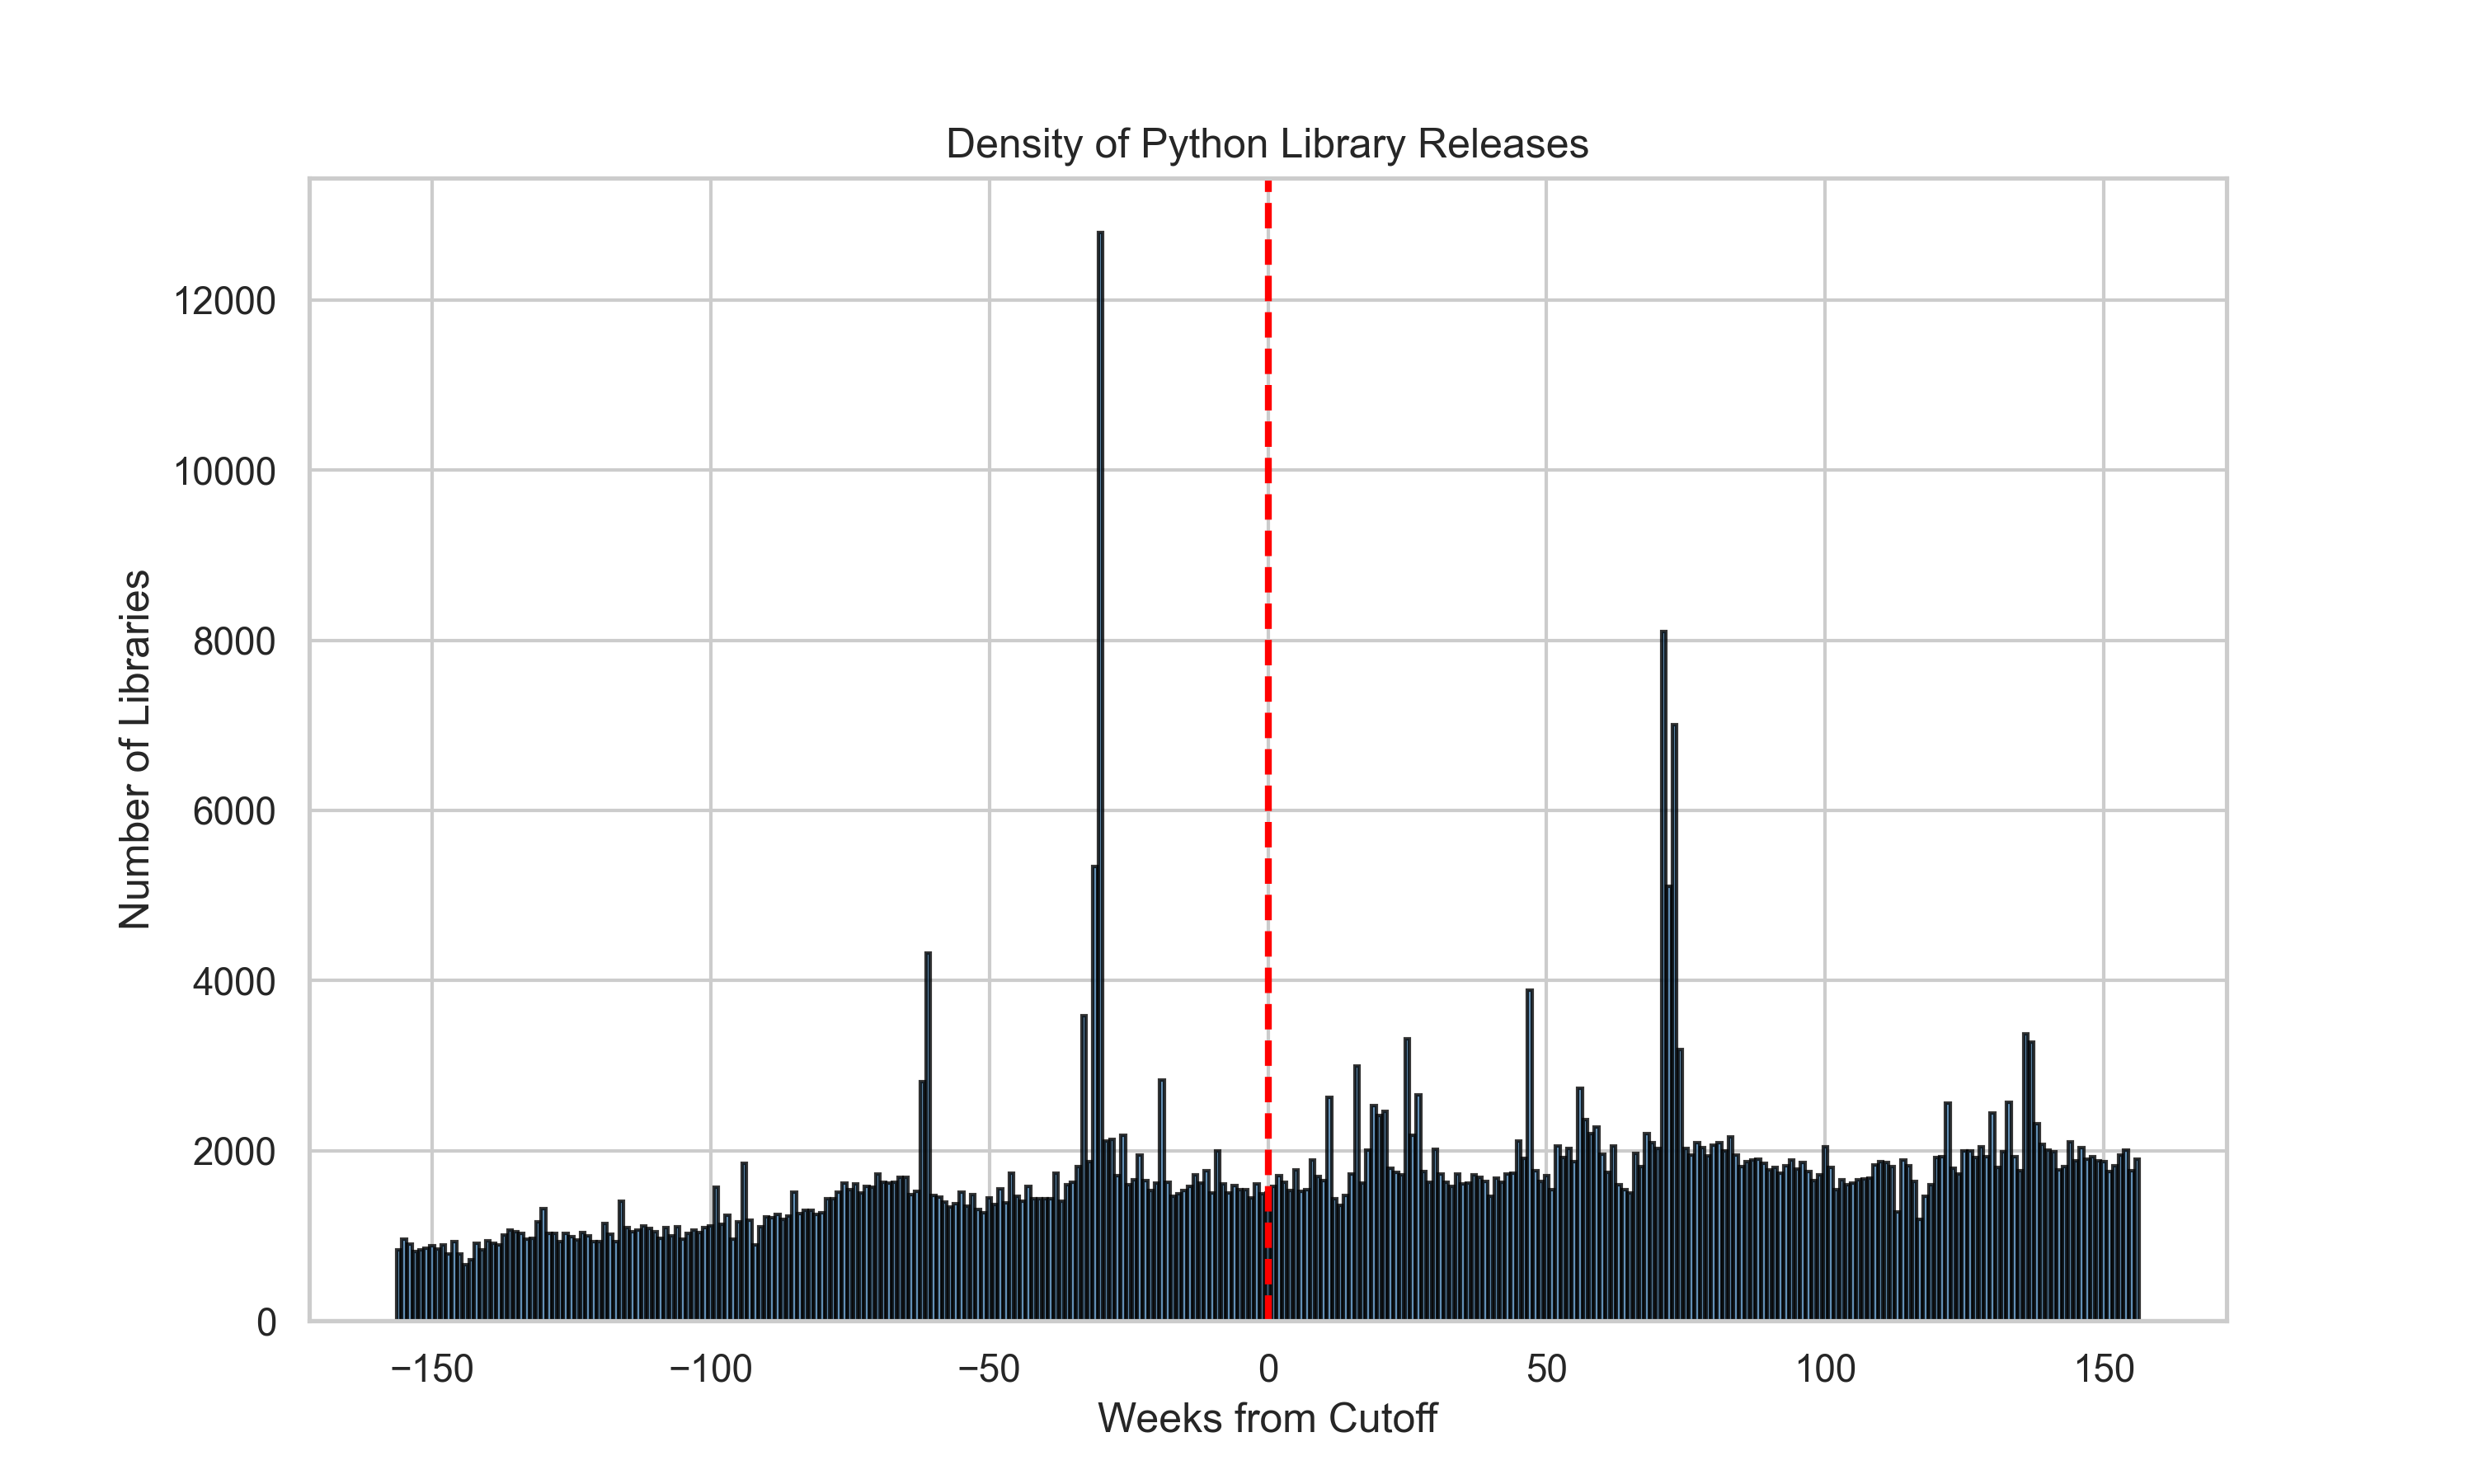
\includegraphics[width=0.85\textwidth]{results/figures/density_dist_to_cutoff.png}
\caption{Density of library releases by week relative to the September 2021 cutoff. The dashed red line marks the cutoff. No systematic bunching is evident at the boundary, consistent with the assumption that release timing is not strategically manipulated around the LLM training cutoff.}\label{fig:density}
\end{figure}

Figure~\ref{fig:density} displays the density of library release dates relative to the September 2021 cutoff. There is no visible discontinuity at the boundary, supporting the identifying assumption that library developers did not systematically time releases around the LLM knowledge cutoff.

\section{Measurement Limitations}\label{sec:data-limitations}
\textbf{Release date proxy.} The first observed download week is a noisy proxy for actual release date. A package may exist on PyPI (or as a GitHub repository) before generating any downloads. If this pre-observation delay is longer for post-cutoff packages — plausible if early adoption is suppressed — the running variable is biased toward zero and the estimated effect is attenuated. This is a conservative bias.

\textbf{PyPI download inflation.} PyPI download counts include automated CI/CD pipeline pulls, mirror syncs, and bot traffic. Raw counts therefore overstate genuine human adoption. The log transformation mitigates the influence of extreme values, but the level of any individual package's downloads cannot be taken as a direct measure of developer intent. This limitation affects levels, not discontinuities, as long as automated download patterns are smooth across the cutoff.

\textbf{GitHub coverage and selection.} The GitHub panel covers a non-random subset of the PyPI universe. Libraries with higher visibility, more active communities, and more GitHub-hosted dependent projects are over-represented. The 5.3\% match rate for the 2021 cohort implies that GitHub-based estimates apply to a selected — and likely more prominent — slice of the library population than PyPI-based estimates. Generalizing from the GitHub subsample to the full PyPI universe requires caution.

\textbf{AI score endogeneity.} The commit-level AI score used to construct the mechanism moderator (\texttt{avg\_ai\_score\_52wk}) is measured over the 52 weeks following release. A library that is suppressed by the LLM cutoff will attract fewer imports overall, and specifically fewer AI-generated imports, because it is less known to LLMs. The moderator therefore partly reflects treatment itself. This endogeneity concern applies only to the exploratory mechanism test and is explicitly acknowledged there. It does not affect the PyPI or GitHub diffusion outcomes, which are the basis for causal inference.

\textbf{Package identity.} Name normalization collapses variants of the same package name but cannot identify library forks, renames, or namespace transfers. A library that was substantially renamed after release would have its pre- and post-rename download histories treated as separate packages. The direction of bias from this error is ambiguous and likely small in aggregate.

% ------------------------------------------------------------------
% Chapter 4
% ------------------------------------------------------------------
\chapter{Empirical Design}\label{ch:methods}

\section{Overview}\label{sec:methods-overview}
This paper uses a Regression Discontinuity Design \citep[RDD;][]{imbens2008regression, lee2010regression} to identify whether Python libraries released shortly before the September 2021 LLM training cutoff diffuse more widely than libraries released shortly after it. The core identifying assumption is that, absent the cutoff, the expected diffusion trajectory of libraries released just before and just after the boundary would have been continuous. Any discrete jump at the cutoff is then attributed to differential LLM knowledge representation.

The baseline design is augmented with a Difference-in-Discontinuities (Diff-in-RDD) strategy that uses three pre-LLM release cohorts (2018–2020) as placebo controls, netting out seasonal variation and any secular trend in the September release calendar. A mechanism test based on AI-scored GitHub commits is implemented as an exploratory extension.

\section{Running Variable and Cutoff Date}\label{sec:methods-running}
The running variable $X_i$ is the release timing of library $i$, measured in weeks relative to the LLM training cutoff. The cutoff date is September 27, 2021, the documented knowledge cutoff for the GPT-3.5 and GPT-4 model families \citep{openai2023gpt4}. Libraries released before this date are, in principle, candidates for inclusion in the pretrained knowledge of these models; libraries released after it are not.

Release timing is operationalized as the first calendar week in which a library recorded at least one PyPI download. This definition is preferred over metadata-reported release dates for three reasons:
\begin{enumerate}
    \item Metadata dates are frequently missing or incorrect in the PyPI registry.
    \item The first observed download week is reproducible from the download panel and requires no external data source.
    \item The first download week is conceptually appropriate: it marks the moment a library becomes observable to the developer community.
\end{enumerate}

The running variable is expressed as $X_i = w_i - c$, where $w_i$ is the first observed download week of library $i$ and $c$ is the week containing September 27, 2021. By construction, $X_i < 0$ for pre-cutoff libraries and $X_i \geq 0$ for post-cutoff libraries.

\subsubsection*{Measurement threats}
Three threats to running variable validity are acknowledged:
\begin{itemize}
    \item Heaping: If developers systematically time releases to calendar milestones, the density of $X_i$ may show non-smooth bunching. Density tests based on \citet{mccrary2008manipulation} are reported.
    \item Delayed observation: A library may exist before its first download, causing $X_i$ to overstate recency. If post-cutoff libraries are suppressed early, this creates a conservative bias toward zero.
    \item Ambiguous inclusion: The exact training data boundary is uncertain. This is addressed by the donut exclusion described in Section~\ref{sec:methods-donut}.
\end{itemize}

\section{Treatment Assignment and Estimand}\label{sec:methods-treatment}
Treatment is defined as follows. Library $i$ is assigned to the post-cutoff group ($D_i = 1$) if $X_i \geq 0$, and to the pre-cutoff group ($D_i = 0$) if $X_i < 0$.

The quantity of interest is the Local Average Treatment Effect at the cutoff (LATE):
$$\tau = \lim_{x \downarrow 0} \mathbb{E}[Y_i \mid X_i = x] - \lim_{x \uparrow 0} \mathbb{E}[Y_i \mid X_i = x]$$
where $Y_i$ is a measure of library diffusion.

\section{Donut Exclusion}\label{sec:methods-donut}
Libraries released within approximately eight weeks before the cutoff occupy an ambiguous zone due to data pipeline lags and crawl schedules. The primary specification applies an asymmetric 9-week donut exclusion, dropping libraries with $X_i \in [-8, 0]$. 

The donut is asymmetric because the post-cutoff boundary is definitionally clean: any library released after September 27, 2021 is excluded from the training corpus. As a robustness check, a symmetric $\pm 4$-week donut is also estimated.

\section{Outcome Variables}\label{sec:methods-outcomes}
\subsubsection*{PyPI downloads}
The primary outcome is the cumulative count of PyPI downloads, measured in $\log(1 + \text{downloads})$. Three horizons are used:
\begin{itemize}
    \item 52-week cumulative downloads: Primary long-run outcome.
    \item Post-AI cumulative downloads: All downloads from November 28, 2022 onward. Designed to isolate the activation window after ChatGPT became a mass interface.
    \item 26-week cumulative downloads: Used for the covariate balance analysis.
\end{itemize}

The 52-week outcome is \textit{horizon-normalized}: every library is measured over the same relative window regardless of release date. The post-AI outcome is instead anchored in \textit{calendar time}: it captures all downloads since a fixed date, meaning the accumulation window grows as the data extend. This has two implications. First, the post-AI estimate is a snapshot; it would yield a different (likely larger) coefficient if re-estimated with data collected six months later. Second, libraries released at different distances from the cutoff have been alive for different durations when the post-AI window opens, introducing a smooth age gradient. The local linear specification absorbs this gradient through its slope terms; the discontinuity estimate captures only the discrete jump at the cutoff, not the continuous age difference. The two outcome types are complementary: the horizon-normalized measure ensures comparability, while the calendar-anchored measure directly tests whether the gap activates after LLMs become widely deployed.

\subsubsection*{GitHub imports}
A secondary outcome is the cumulative count of GitHub code files importing library $i$, also transformed as $\log(1 + \text{imports})$. The implementation gap-comparing the discontinuity in GitHub imports vs. PyPI downloads-serves as the primary mechanism test.

\section{Main Estimator: Local Linear RDD}\label{sec:methods-rdd}
The main estimating equation is a local linear regression on each side of the cutoff:
$$Y_i = \alpha + \tau D_i + \beta_1 X_i + \beta_2 D_i \cdot X_i + \varepsilon_i$$
estimated using observations within a bandwidth $h$ ($|X_i| \leq h$). Estimates use the \texttt{rdrobust} package \citep{calonico2014robust, calonico2020rdrobust} with:
\begin{itemize}
    \item Polynomial order: $p = 1$ (local linear).
    \item Bandwidth: $h = 13$ weeks, consistent with the Diff-in-RDD specification. Stability across wider bandwidths is verified in Section~\ref{subsec:rob-bw}.
    \item Inference: Robust bias-corrected (rbc) confidence intervals.
    \item Kernel: Triangular.
\end{itemize}

\section{Identification Strategy: Difference-in-Discontinuities}\label{sec:methods-diffrdd}
The main RDD identifies $\tau$ under the assumption that counterfactual diffusion is continuous at the cutoff. A threat to this assumption is \textbf{calendar confounding}: the September window may differ from other months in ways that affect diffusion independently of LLM cutoffs, for example, seasonal variation in developer activity or a concentration of high-quality releases in the late summer academic cycle. To address this, the primary causal specification is a Difference-in-Discontinuities (Diff-in-RDD) design \citep{grembi2016fiscal}.

Three cohorts of libraries (released in 2018, 2019, and 2020, before any LLM with documented training cutoffs was publicly deployed) serve as placebo controls. The Diff-in-RDD estimator extracts the 2021-specific excess jump:
$$\hat{\tau}^{\text{Diff-in-RDD}} = \hat{\tau}_{2021} - \frac{1}{3}\sum_{t \in \{2018,2019,2020\}} \hat{\tau}_t$$
where $\hat{\tau}_t$ is the estimated RDD discontinuity for cohort $t$, each estimated at the same calendar position (the Monday-aligned week nearest September~27 in year $t$).

\textbf{Implementation.} The Diff-in-RDD is estimated as a stacked weighted least squares (WLS) regression. Pooling all four cohort years, the specification is:
$$\log(1 + Y_{it}) = \alpha + \beta_1 D_{it} + \beta_2 \mathbb{1}_{2021} + \beta_3 (D_{it} \times \mathbb{1}_{2021}) + g(X_{it}, D_{it}, \mathbb{1}_{2021}) + \varepsilon_{it}$$
where $D_{it} = \mathbb{1}(X_{it} \geq 0)$ is the post-cutoff indicator, $\mathbb{1}_{2021}$ is an indicator for the 2021 cohort, and $g(\cdot)$ contains the running variable $X_{it}$ and its full set of interactions with $D_{it}$ and $\mathbb{1}_{2021}$, allowing separate slopes on each side of the cutoff in each cohort. Triangular kernel weights $w_i = 1 - |X_i|/h$ are applied, with bandwidth $h = 13$ weeks. The coefficient of interest is $\beta_3$: the excess discontinuity in the 2021 cohort relative to the placebo average.

Standard errors are clustered at the \textbf{year-by-week} level (i.e., each unique combination of cohort year and running variable value forms a cluster). With four cohort years and approximately 18 effective running variable values within bandwidth (after donut exclusion), this yields roughly 72 clusters, providing sufficient mass for cluster-robust inference.

\textbf{Identifying assumption.} The Diff-in-RDD identifies the causal effect under the assumption that the 2021 discontinuity, conditional on the 2018--2020 baseline discontinuity, would be zero in the absence of the LLM training cutoff. This is weaker than the standard RDD continuity assumption: it does not require that September is identical to other months; only that any September-specific pattern is stable across years. The validity of this parallel-trends assumption is supported by the observation that estimated placebo discontinuities in 2018--2020 are individually small and jointly insignificant.

\section{Success Tiers and the Barrier-to-Entry Test}\label{sec:methods-barrier}
Three tiers are defined based on cumulative 26-week PyPI downloads (pre-ChatGPT window):
\begin{itemize}
    \item Broad: $\geq 10$ downloads.
    \item Successful: $\geq 500$ downloads.
    \item Superstar: $\geq 1,000$ downloads.
\end{itemize}
The barrier-to-entry test uses a Linear Probability Model (LPM) to estimate the discontinuity in the probability of reaching the Successful tier.

\section{Mechanism Test: AI Exposure Moderation}\label{sec:methods-mechanism}
A direct mechanism test examines whether suppression is heterogeneous by AI exposure intensity:
$$Y_i = \alpha + \tau D_i + \gamma \cdot \text{HighAI}_i + \delta \cdot (D_i \times \text{HighAI}_i) + f(X_i) + \varepsilon_i$$
The coefficient of interest is $\delta$, representing the differential suppression effect for libraries frequently found in AI-generated code.

\section{Robustness Checks}\label{sec:methods-robustness}

\subsection{Bandwidth Sensitivity}\label{subsec:rob-bw}
The stability of estimates is evaluated across a range of bandwidths $h \in \{13, 15, 20, 26, 30, 40\}$ weeks. The single-year 2021 RDD showed sensitivity to bandwidth choice, and the MSE-optimal bandwidth selection in \texttt{rdrobust} failed numerically for the large-$N$ PyPI specifications. This sensitivity provided the empirical justification for the Diff-in-RDD strategy, which remains stable and significant across these same bandwidth choices by using previous years (2018--2020) as a counterfactual for seasonal release patterns.

\subsection{Donut Specification}\label{subsec:rob-donut}
The primary design uses an asymmetric 9-week donut (excluding the period from late July to September 27, 2021). This is motivated by the substantive uncertainty of whether libraries released in the final weeks before the cutoff were successfully scraped and processed into the model's training set. To ensure this specific exclusion does not drive the result, a standard symmetric $\pm 4$-week donut is also reported. The effect remains robust (e.g., $Estimate = -4.35, p < 0.001$ for the Successful tier), suggesting the Knowledge Wall is not an artifact of the specific exclusion window.

\subsection{Placebo Cutoffs}\label{subsec:rob-placebo}
The RDD is replicated for the 2018, 2019, and 2020 cohorts using the same relative calendar dates. These placebo years lack a major LLM training cutoff. The absence of significant discontinuities in these years helps rule out alternative explanations such as annual seasonality in Python library releases (e.g., end-of-quarter or pre-conference release spikes) that could otherwise be mistaken for a treatment effect.

\subsection{Density Test}\label{subsec:rob-density}
A core RDD assumption is that there is no sorting or manipulation of the running variable around the cutoff. In this context, it is implausible that developers in mid-2021 could have anticipated the exact September 27 training cutoff of models like GPT-4 or the subsequent mass adoption of ChatGPT. Visual density plots confirm a smooth distribution of library releases across the threshold, with no evidence of clustering on the pre-cutoff side.

\subsection{Covariate Balance}\label{subsec:rob-covariates}
Pre-treatment covariate balance is assessed using the pre-AI success rate RDD reported in Section~\ref{sec:results-barrier}: if libraries on either side of the cutoff are comparable in human-evaluated quality before ChatGPT, quality sorting cannot explain the post-AI discontinuity.

\section{Permutation Inference}\label{sec:methods-permutation}
A non-parametric permutation test provides a distribution-free assessment of whether the discontinuity at the September 2021 cutoff is unusual relative to what would be observed at arbitrary dates. Following the moving-cutoff logic common in the causal inference literature \citep[e.g.,][]{dell2010persistent}, the primary RDD model is re-estimated using 157 alternative placebo Mondays between January 2019 and January 2022.

For each iteration, a hypothetical treatment is defined based on a pseudo-cutoff date ($c'$), the running variable is calculated relative to that date, and the local linear discontinuity is estimated for the primary outcome (cumulative 52-week downloads). This procedure yields an empirical null distribution of RDD coefficients. The empirical $p$-value is calculated as:
$$p_{perm} = \frac{1}{N} \sum_{i=1}^{N} \mathbb{I}(|\hat{\beta}_{placebo, i}| \geq |\hat{\beta}_{true}|)$$

Results of the permutation test are reported in Section~\ref{sec:results-robustness}.

% ------------------------------------------------------------------
% Chapter 5
% ------------------------------------------------------------------
\chapter{Results}\label{ch:results}

\section{Sequence of Evidence}\label{sec:results-sequence}
The empirical evidence is presented in five steps. First, the raw discontinuity in the 2021 cohort establishes that a jump exists at the September 2021 boundary. Second, the Difference-in-Discontinuities design establishes that the 2021 jump is anomalously small relative to historical norms — constituting a net suppression. Third, the barrier-to-entry analysis shows that the suppression operates at the level of library emergence, not only diffusion levels. Fourth, the implementation gap establishes that suppression is amplified in AI-generated code relative to general downloads. Fifth, the mechanism moderation test and bandwidth sensitivity analysis complete the robustness picture.

Throughout, descriptive comparisons are presented before formal estimates, and magnitude interpretations are given alongside statistical significance.

\section{Descriptive Patterns}\label{sec:results-descriptive}
Before estimating discontinuities, it is useful to characterize the distribution of the main outcomes. Table~\ref{tab:descriptive} reports summary statistics for the primary outcome variables in the 2021 cohort.

\begin{table}[ht]
\centering
\caption{Descriptive Statistics: 2021 Cohort}\label{tab:descriptive}
\small
\begin{tabular}{lrrrrrr}
\toprule
\textbf{Variable} & \textbf{N} & \textbf{Mean} & \textbf{Median} & \textbf{SD} & \textbf{p10} & \textbf{p90} \\ \midrule
\multicolumn{7}{l}{\textit{PyPI Downloads (Broad tier, min 10)}} \\
\quad 52-week downloads & 527{,}361 & 25{,}661 & 2{,}307 & 1{,}439{,}110 & 96 & 15{,}456 \\
\quad Post-AI downloads  & 527{,}361 & 748{,}094 & 4{,}005 & 49{,}081{,}592 & 11 & 44{,}113 \\[4pt]
\multicolumn{7}{l}{\textit{GitHub Imports (matched subsample)}} \\
\quad 52-week imports     & 28{,}243 & 147.1 & 2.0 & 5{,}077.0 & 0 & 98 \\
\quad Post-AI imports     & 28{,}243 & 318.4 & 7.0 & 6{,}721.7 & 0 & 196 \\[4pt]
\multicolumn{7}{l}{\textit{AI Exposure Score (matched subsample)}} \\
\quad avg\_ai\_score\_52wk & 8{,}566 & 0.272 & 0.232 & 0.391 & $-0.217$ & 0.878 \\
\bottomrule
\end{tabular}
\begin{tablenotes}
\small
\item \textit{Notes:} Statistics computed on the full 2021 analysis sample within $h = 13$ weeks of the cutoff, excluding the 9-week donut. Downloads and imports are in levels (not logged). AI exposure scores are available only for the GitHub-matched subsample with non-zero commit activity. The score is a bias-corrected estimate and is not bounded to $[0,1]$; negative values arise when the raw classification rate falls below the classifier's estimated false positive rate.
\end{tablenotes}
\end{table}

The distribution of 52-week cumulative PyPI downloads is heavily right-skewed: the median library in the Broad tier records substantially fewer downloads than the mean, and the top decile accounts for the majority of total download volume. After the $\log(1 + \text{downloads})$ transformation, the distribution is approximately unimodal. GitHub import counts are even more concentrated: the majority of matched libraries record zero or near-zero AI-era imports, with a small number of high-visibility libraries accounting for most of the observed import mass.

Among libraries released within $\pm 13$ weeks of the September 2021 cutoff (excluding the donut), the unconditional mean of post-AI cumulative downloads is higher for post-cutoff libraries than for pre-cutoff libraries. This raw gap, however, reflects a seasonal pattern common to all cohort years: post-September libraries in general tend to accumulate more downloads in subsequent years, for reasons unrelated to LLM knowledge cutoffs. Identifying the cutoff-specific effect requires netting out this baseline through the Diff-in-RDD design.

\section{Main RDD: Raw Discontinuity at the 2021 Cutoff}\label{sec:results-mainrdd}
Table~\ref{tab:mainrdd} reports the baseline RDD estimates for the 2021 cohort, estimated using \texttt{rdrobust} with bias-corrected local linear regression, triangular kernel, and $h = 13$ weeks. The donut exclusion (weeks $-8$ to $0$) is applied.

\begin{table}[h!]
\centering
\caption{Main RDD Estimates, 2021 Cohort}\label{tab:mainrdd}
\small
\begin{tabular}{llcccc}
\toprule
\textbf{Tier} & \textbf{Outcome} & \textbf{Estimate (log pts)} & \textbf{SE} & \textbf{p-value} & \textbf{N} \\ \midrule
Broad (min 10) & 52-week Downloads & +9.572 & 2.670 & $<$0.001 & 527,361 \\
Broad (min 10) & Post-AI Downloads & +13.103 & 4.494 & 0.004 & 527,361 \\
Successful (min 500) & Post-AI Downloads & $-0.195$ & 3.125 & 0.950 & 407,110 \\ \bottomrule
\end{tabular}
\begin{tablenotes}
\small
\item \textit{Notes:} Bias-corrected robust estimates via \texttt{rdrobust}. Triangular kernel, $h = 13$ weeks, 9-week asymmetric donut. Post-AI downloads are cumulative from November 28, 2022 onward.
\end{tablenotes}
\end{table}

A statistically significant positive discontinuity is visible in the Broad tier: post-cutoff libraries acquire more downloads than pre-cutoff libraries at the boundary, both at the 52-week horizon (+9.6 log points, $p < 0.001$) and in the post-AI activation window (+13.1 log points, $p = 0.004$). The positive sign reflects the direction of the raw jump: post-cutoff libraries, released in autumn and winter 2021, record higher unadjusted download totals than libraries released in the preceding summer months.

The positive raw jump is consistent with a well-documented seasonal pattern in developer software adoption. Second, the positive discontinuity in the Broad tier disappears entirely in the Successful subsample ($-0.195$, $p = 0.950$). This is the first signal of the barrier-to-entry mechanism.

\begin{figure}[ht]
\centering
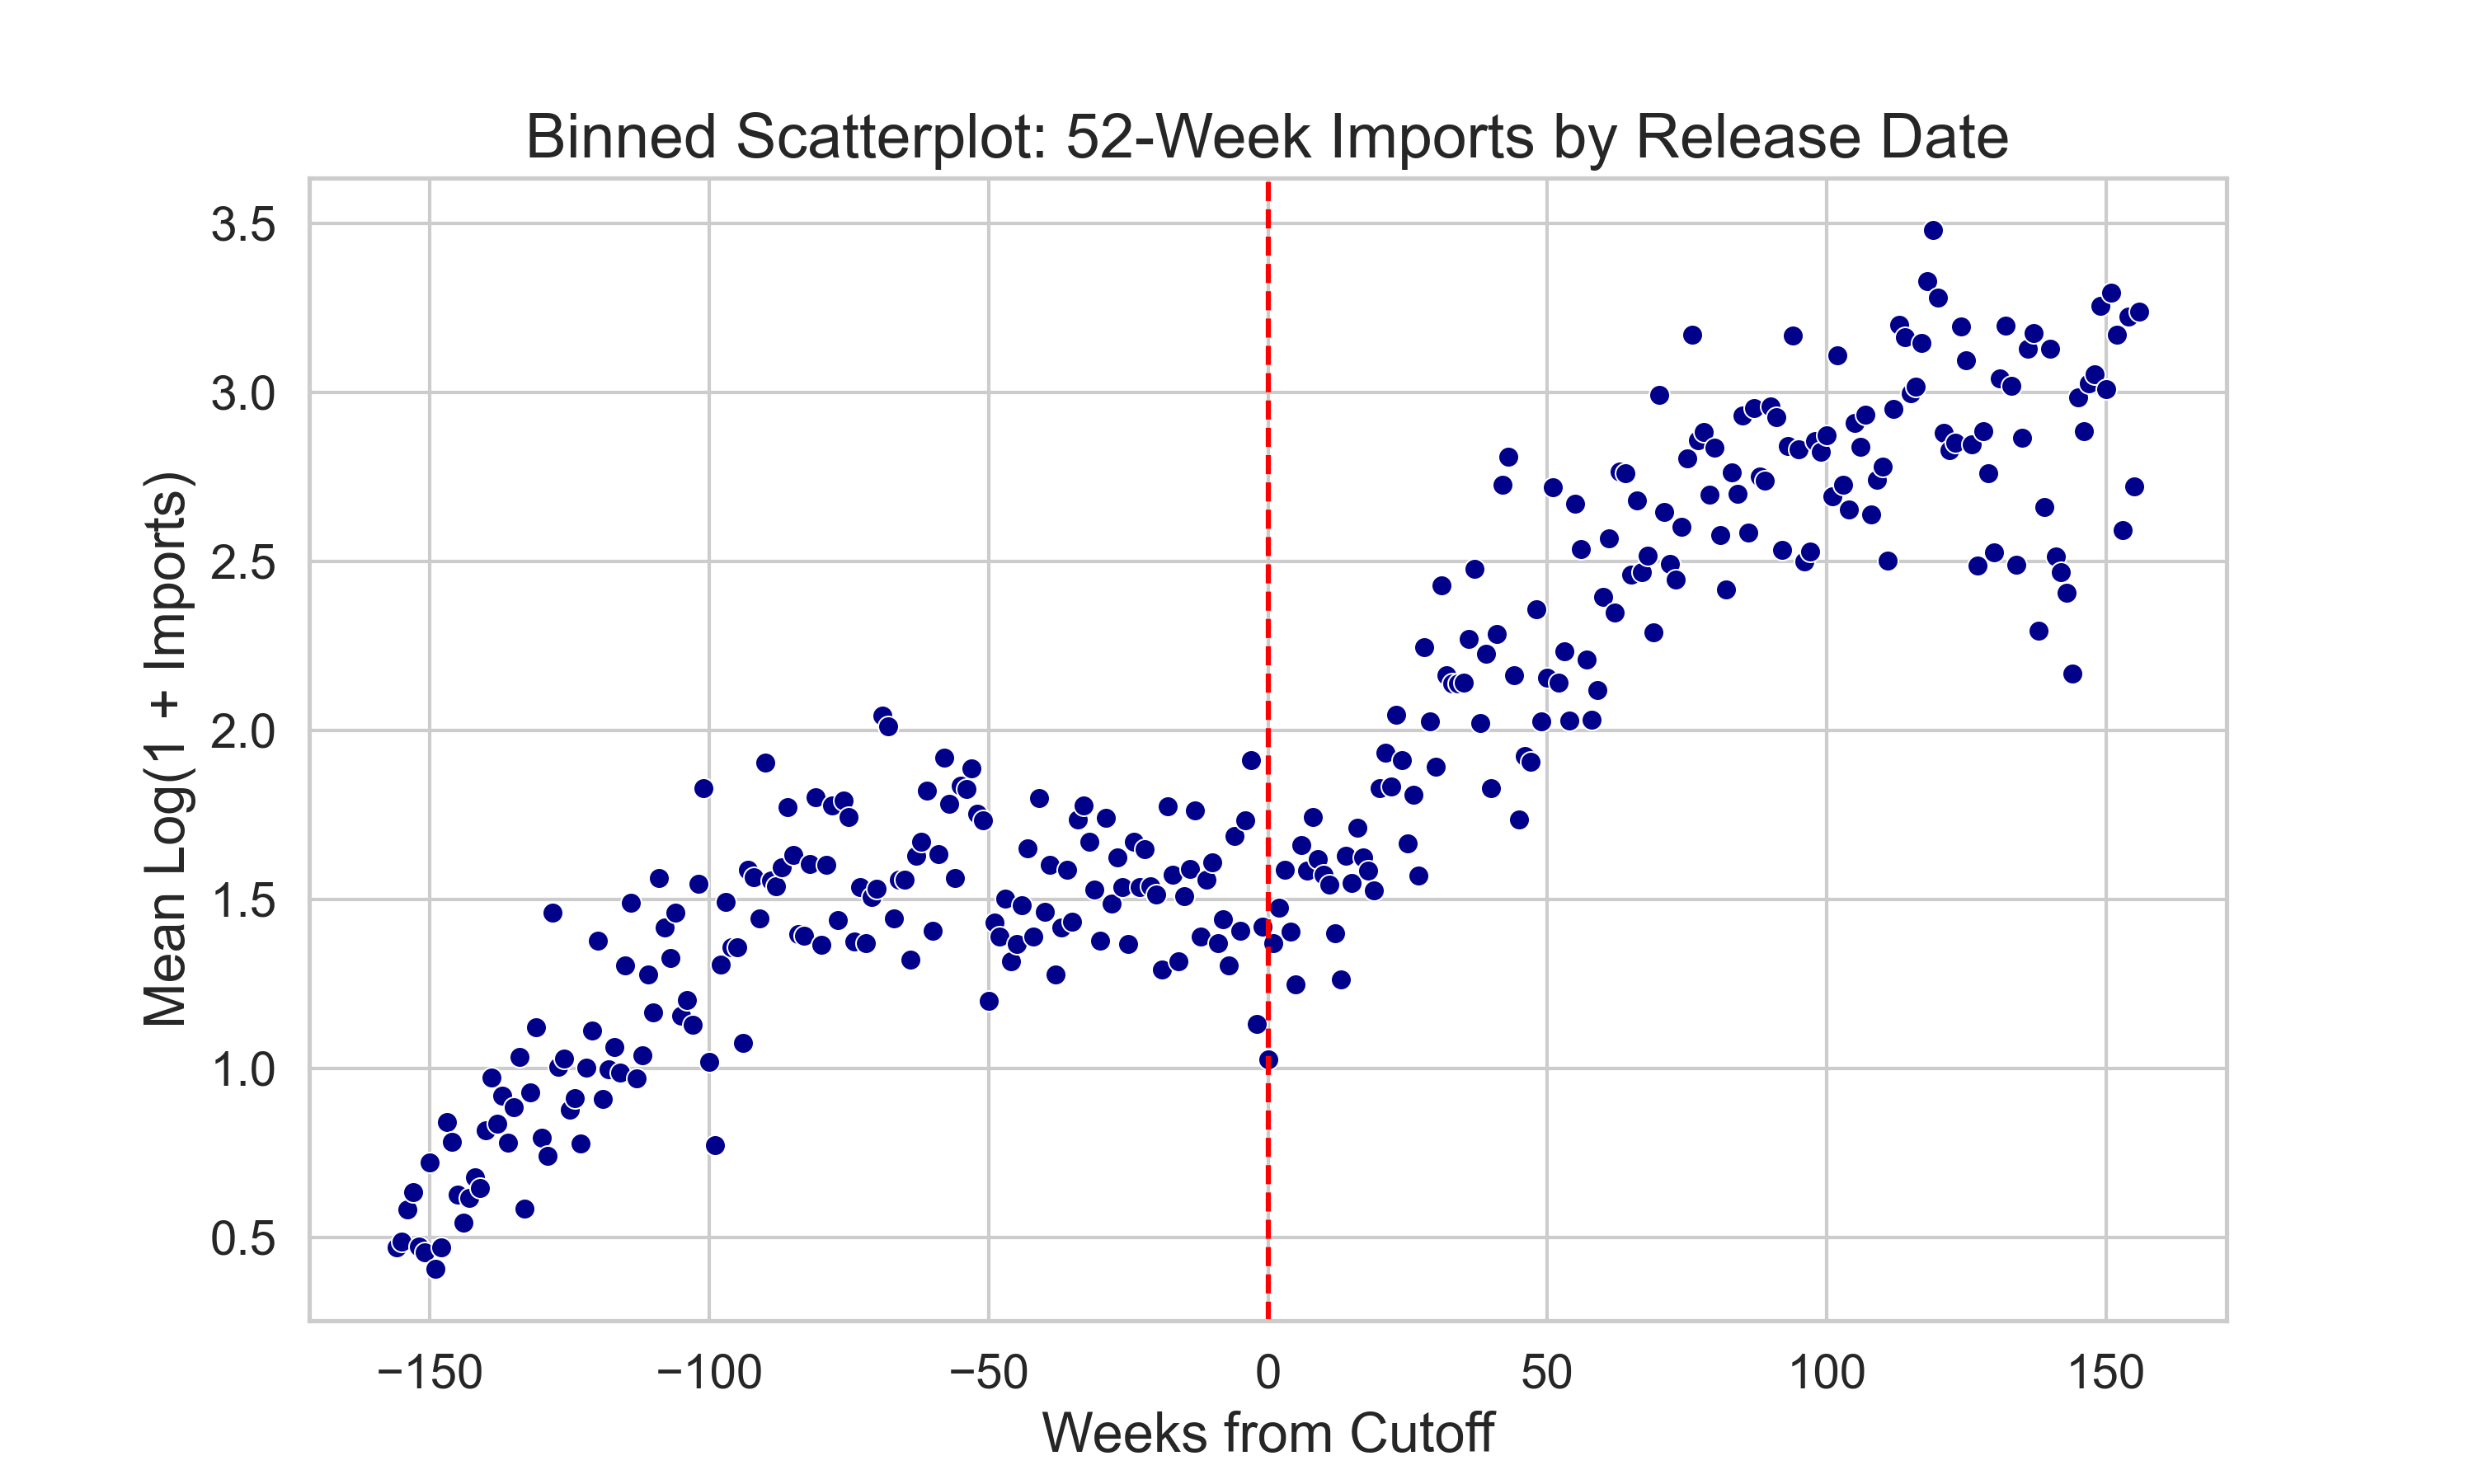
\includegraphics[width=0.85\textwidth]{results/figures/binscatter_log_imports.png}
\caption{Binned scatterplot of $\log(1 + \text{52-week imports})$ by release week relative to the September 2021 cutoff. Each point represents a weekly bin average. The upward trend reflects the secular growth of the Python ecosystem; the discontinuity at the cutoff captures the raw RDD effect, which mixes the Knowledge Wall penalty with the seasonal baseline.}\label{fig:binscatter-imports}
\end{figure}

\section{Causal Identification: Difference-in-Discontinuities}\label{sec:results-diffrdd}
The Diff-in-RDD stacks the 2021 cohort with three placebo cohorts (2018, 2019, 2020), estimates the RDD discontinuity for each year at the same calendar position, and extracts the 2021-specific excess. The excess jump is identified by the interaction term $\hat{\tau}^{2021} - \bar{\hat{\tau}}^{\text{placebo}}$, estimated via WLS.

\begin{table}[h!]
\centering
\caption{Diff-in-RDD Estimates: 2021 Excess Jump}\label{tab:diffrdd}
\small
\begin{tabular}{llcccc}
\toprule
\textbf{Tier} & \textbf{Outcome} & \textbf{Excess Jump (log pts)} & \textbf{Cluster SE} & \textbf{p-value} & \textbf{N} \\ \midrule
Broad (min 10) & Post-AI Downloads & $-9.139$ & 4.425 & 0.039 & 88,001 \\
Successful (min 500) & Post-AI Downloads & $-12.792$ & 4.827 & 0.008 & 75,313 \\
Superstar (min 1000) & Post-AI Downloads & $-0.553$ & 0.492 & 0.261 & 57,931 \\ \bottomrule
\end{tabular}
\begin{tablenotes}
\small
\item \textit{Notes:} WLS with year-by-week clustered standard errors. Triangular kernel, $h = 13$ weeks, 9-week asymmetric donut. Placebo cutoffs at equivalent calendar position in 2018, 2019, and 2020.
\end{tablenotes}
\end{table}

The excess jump is significantly negative for both the Broad ($-9.1$ log points, $p = 0.039$) and Successful ($-12.8$ log points, $p = 0.008$) tiers. Relative to the historical seasonal baseline, post-cutoff libraries in 2021 accumulated approximately 12.8 log points fewer post-AI downloads than pre-cutoff libraries.

The horizon-normalized 52-week outcome also yields a negative Diff-in-RDD for the Successful tier ($-3.7$ log points, $p = 0.026$). This is consistent with the post-AI suppression activating within the 52-week window for libraries released in autumn 2021, whose 52-week accumulation period extends into late 2022 and partially overlaps with the ChatGPT deployment window.

\begin{figure}[ht]
\centering
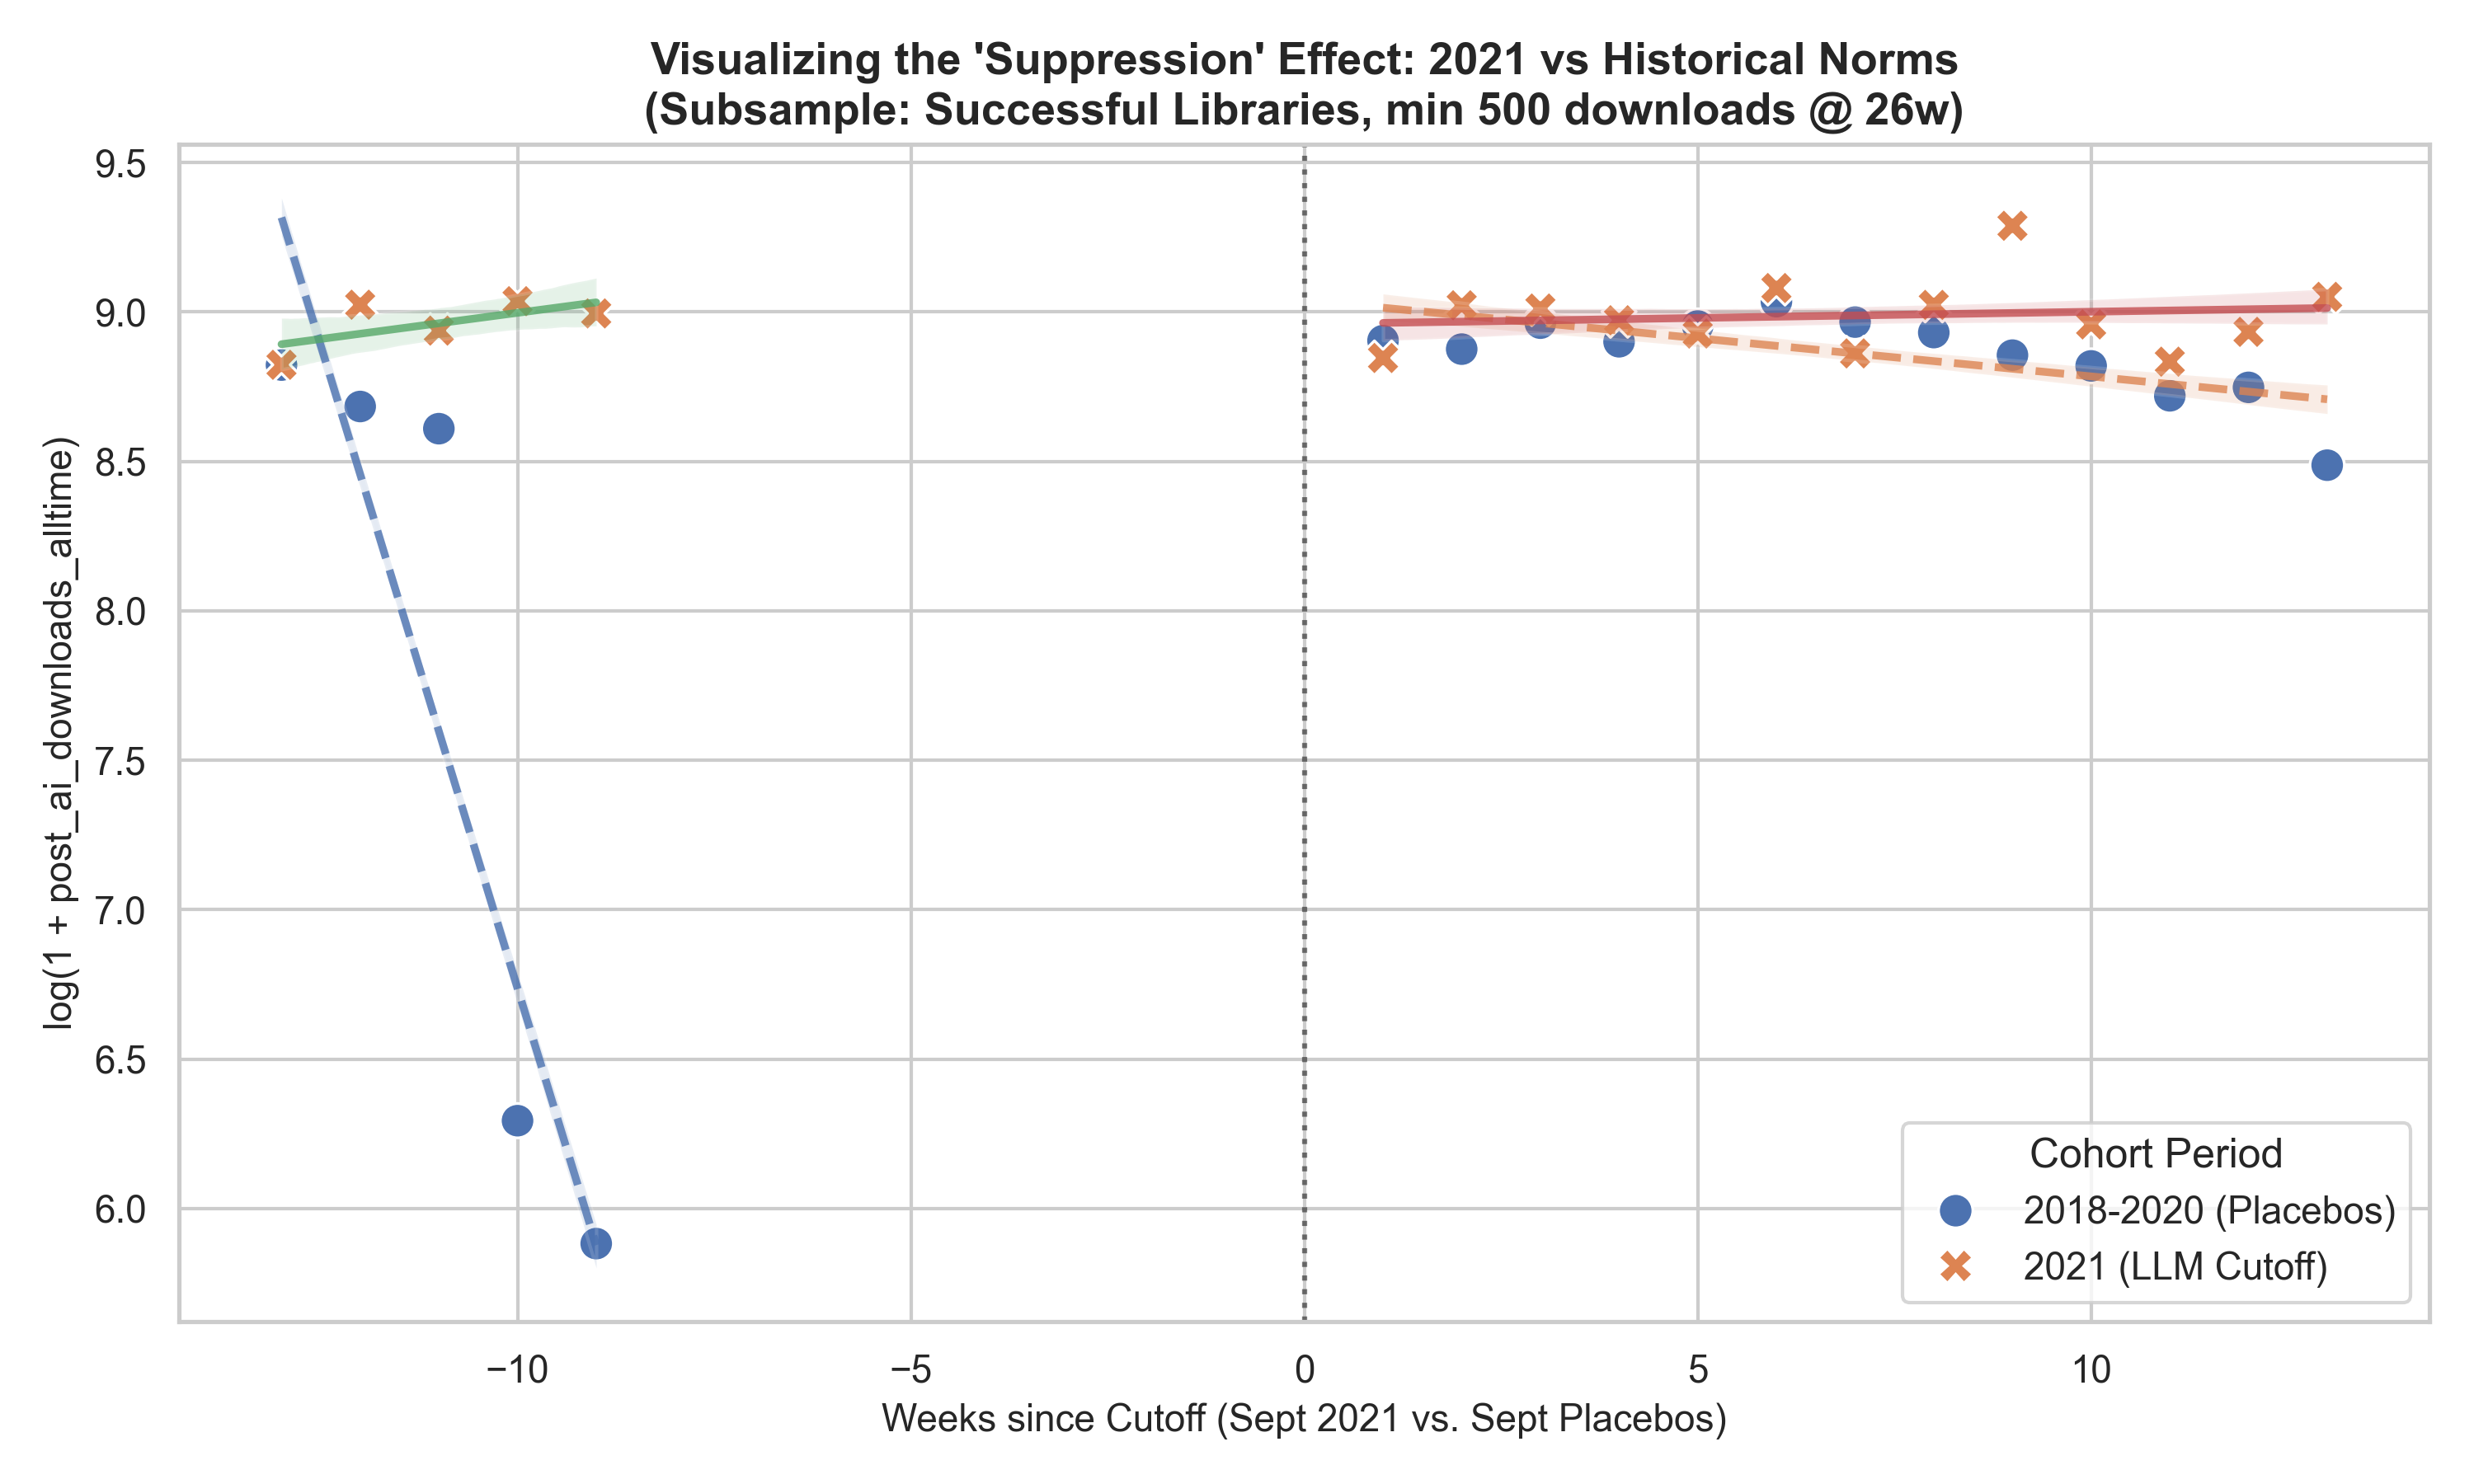
\includegraphics[width=0.85\textwidth]{results/figures/suppression_visual_success_500.png}
\caption{Diff-in-RDD visualization for the Successful tier (min.\ 500 downloads at 26 weeks). Blue circles: pooled 2018--2020 placebo cohorts. Orange crosses: 2021 cohort. Fitted lines show local linear estimates on each side of the cutoff. The 2021 cohort is shifted downward relative to the historical seasonal norm, identifying the Knowledge Wall penalty.}\label{fig:diffrdd-visual}
\end{figure}

\section{Covariate Balance: Pre-AI Success Rates}\label{sec:results-barrier}
Before interpreting the post-AI suppression estimates, it is important to verify that libraries on either side of the cutoff were comparable in their \textit{pre-AI} performance, measured before ChatGPT could have influenced adoption patterns. An RDD with a binary outcome (whether library $i$ crossed the 500-download threshold within its first 26 weeks) tests whether baseline human-developer adoption differs at the cutoff. The 26-week window closes in approximately March 2022 for the 2021 cohort, entirely before ChatGPT.

\begin{table}[ht]
\centering
\caption{Pre-AI Covariate Balance: Probability of Reaching the Successful Tier}\label{tab:barrier}
\small
\begin{tabular}{lcccc}
\toprule
\textbf{Outcome} & \textbf{Estimate (pp)} & \textbf{Robust SE} & \textbf{p-value} & \textbf{N} \\ \midrule
$\Pr(\text{downloads}_{26\text{wk}} \geq 500)$ & $+28.6$ & $3.94$ & $<0.001$ & $78{,}762$ \\ \bottomrule
\end{tabular}
\begin{tablenotes}
\small
\item \textit{Notes:} Linear probability model via \texttt{rdrobust}. Bias-corrected robust estimate. Triangular kernel, $h = 26$ weeks, 9-week asymmetric donut. Positive estimate indicates post-cutoff libraries are \textit{more} likely to reach the threshold.
\end{tablenotes}
\end{table}

Post-cutoff libraries are approximately 29 percentage points \textit{more} likely to reach the Successful tier in their first 26 weeks than pre-cutoff libraries. This pre-AI advantage for post-cutoff libraries likely reflects seasonal patterns in library release and early adoption. Critically, it implies that the post-AI suppression documented in Tables~\ref{tab:diffrdd} and~\ref{tab:github-rdd} is \textit{conservative}: post-cutoff libraries that start with a pre-AI advantage nevertheless fall behind once LLMs become a mass interface. The Diff-in-RDD design, which nets out such seasonal baselines, remains the appropriate estimator for the causal suppression effect.

\section{The Implementation Gap: GitHub versus PyPI}\label{sec:results-github}
A cleaner test of the LLM-mediated channel uses GitHub import counts. Table~\ref{tab:github-rdd} reports \texttt{rdrobust} estimates for the GitHub-matched subsample ($N = 28,243$).

\begin{table}[h!]
\centering
\caption{Main RDD Estimates: GitHub Implementation}\label{tab:github-rdd}
\small
\begin{tabular}{lcccc}
\toprule
\textbf{Outcome} & \textbf{Estimate (log pts)} & \textbf{SE} & \textbf{p-value} & \textbf{N} \\ \midrule
52-week Imports & +11.554 & 10.778 & 0.284 & 28,243 \\
GPT-4 Era Imports & +23.256 & 11.541 & 0.044 & 28,243 \\
Post-AI Imports & +26.767 & 10.932 & 0.014 & 28,243 \\
All-Time Imports & +27.863 & 9.987 & 0.005 & 28,243 \\ \bottomrule
\end{tabular}
\end{table}

The all-time estimate (+27.9 log points) is approximately twice the corresponding PyPI post-AI estimate (+13.1 log points). However, this comparison should be interpreted with caution: the PyPI estimate uses the full Broad-tier sample ($N = 527{,}361$), while the GitHub estimate uses a 5.3\% matched subsample ($N = 28{,}243$) that over-represents prominent, widely-used libraries. The larger GitHub coefficient may partly reflect sample composition (more visible libraries have more to lose from reduced discoverability) rather than a pure difference between the implementation and discovery channels. With this caveat, the amplification is consistent with LLM-steered code generation as the operative channel. Figure~\ref{fig:horizon-coef} shows that the estimated discontinuity grows monotonically from the 52-week horizon through the all-time horizon, consistent with the activation hypothesis: the gap is dormant at release and emerges only after LLMs become a mass interface.

\begin{figure}[ht]
\centering
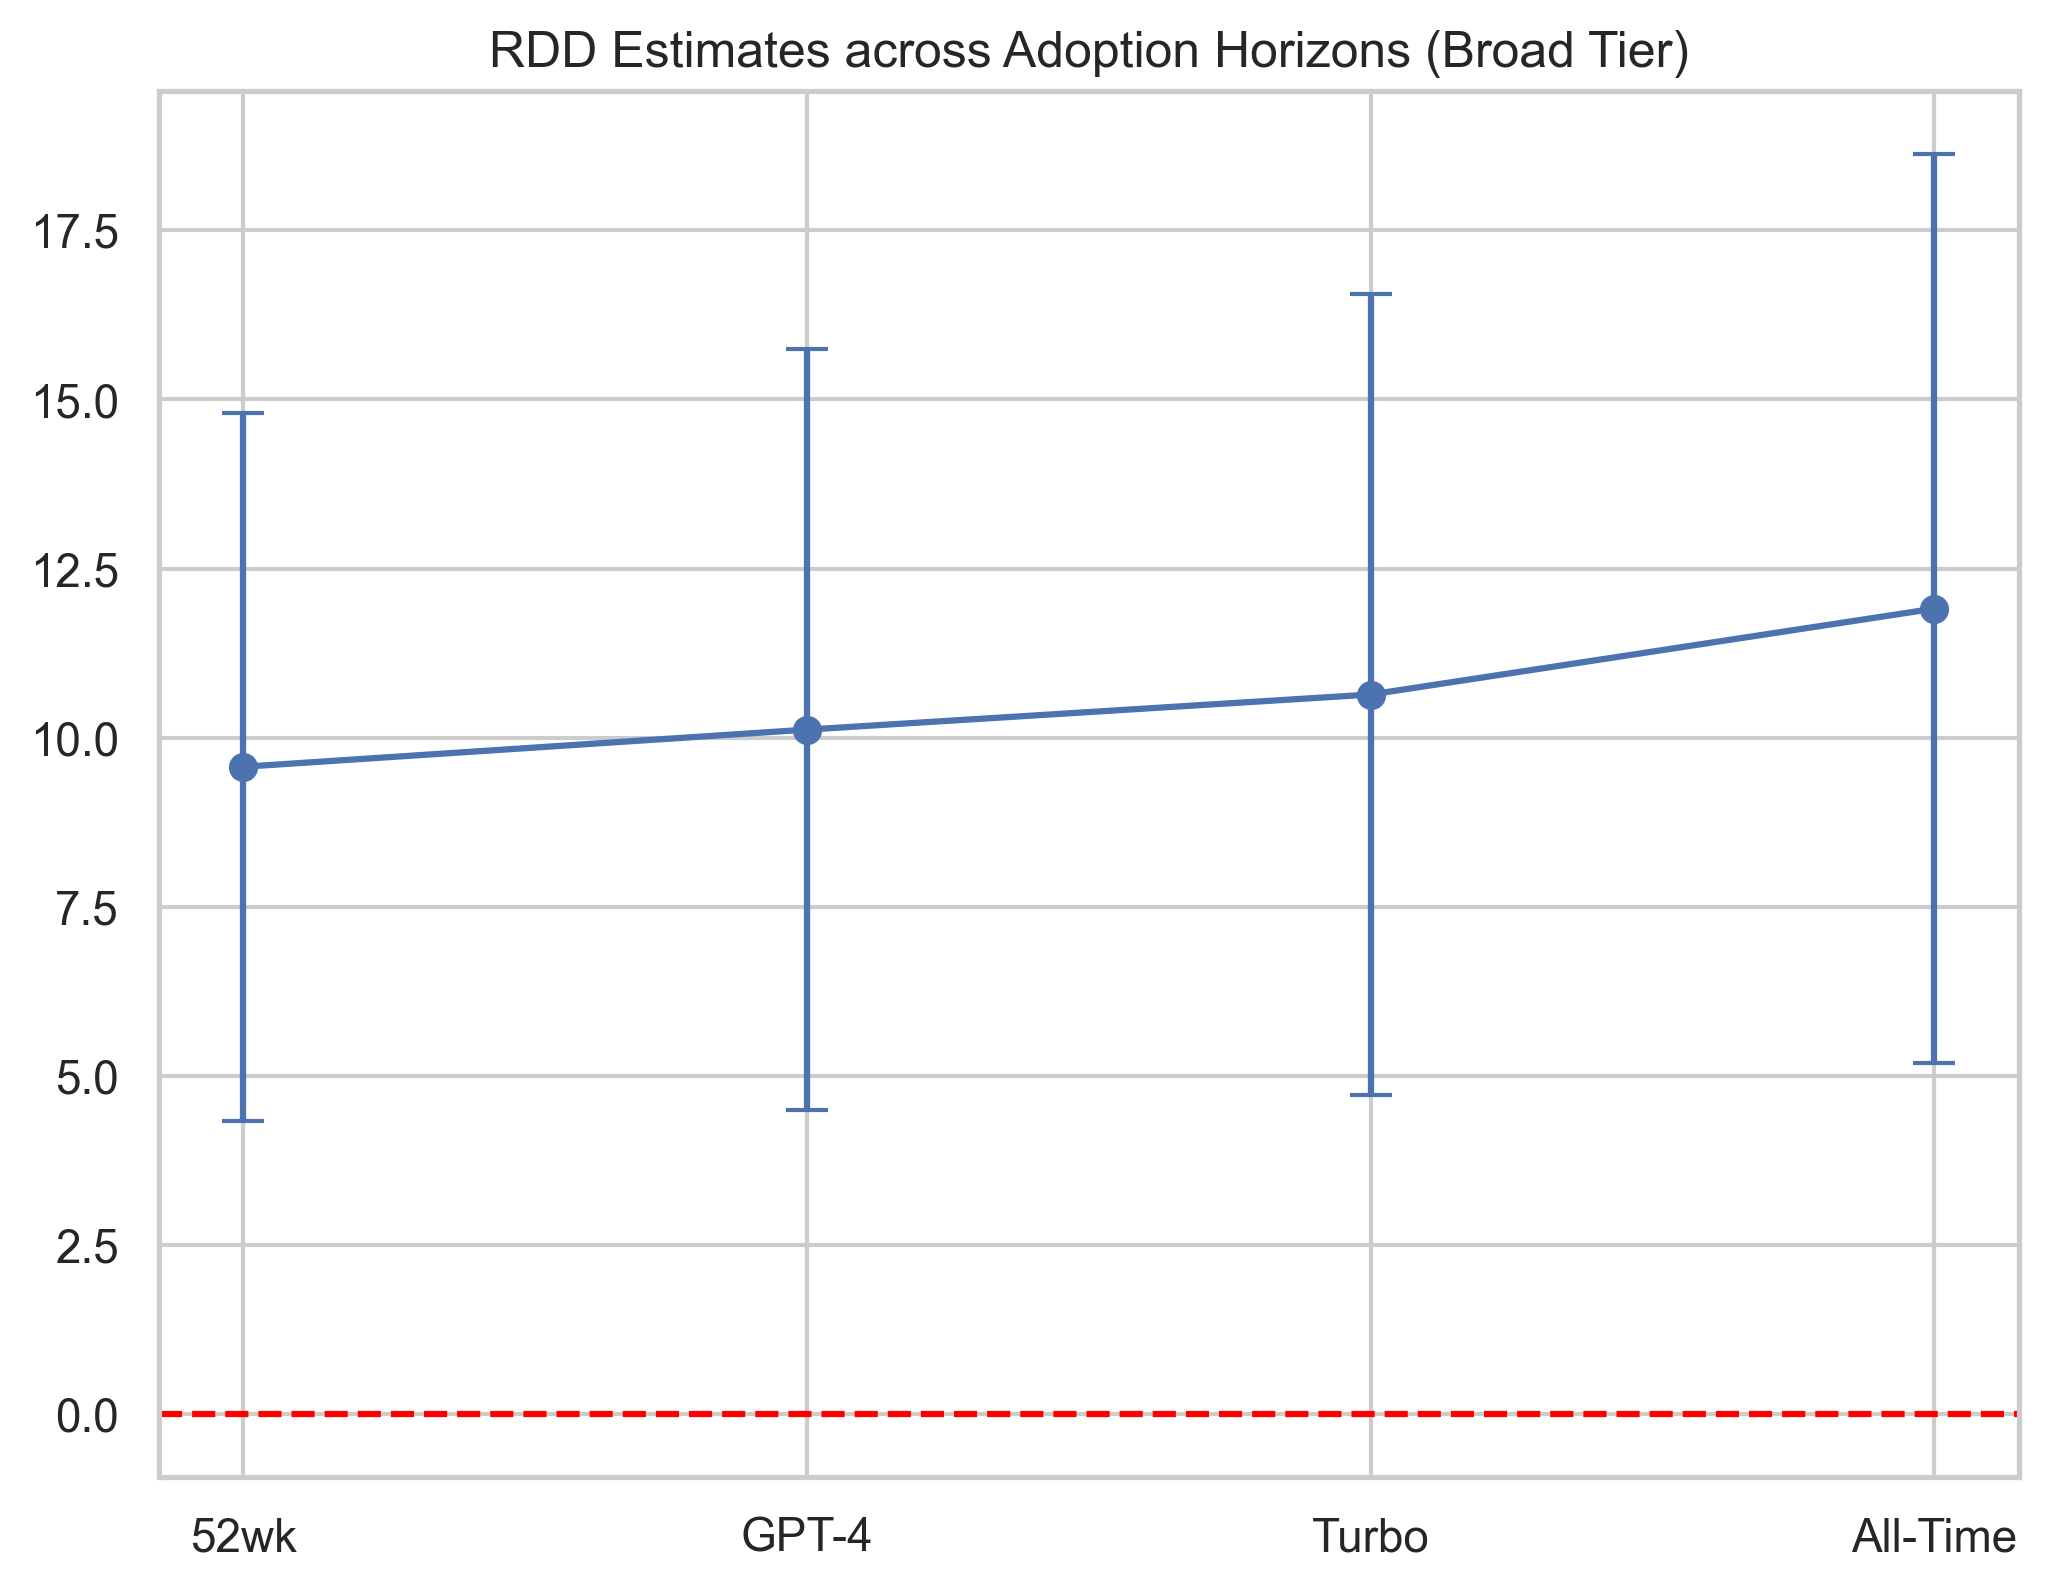
\includegraphics[width=0.7\textwidth]{results/figures/rdd_horizon_coefficients.png}
\caption{RDD point estimates for PyPI downloads across adoption horizons (Broad tier). Vertical bars are 95\% robust confidence intervals. The estimate grows from the 52-week horizon (mostly pre-ChatGPT) through the all-time horizon, consistent with the activation of the Knowledge Wall after November 2022.}\label{fig:horizon-coef}
\end{figure}

\begin{figure}[ht]
\centering
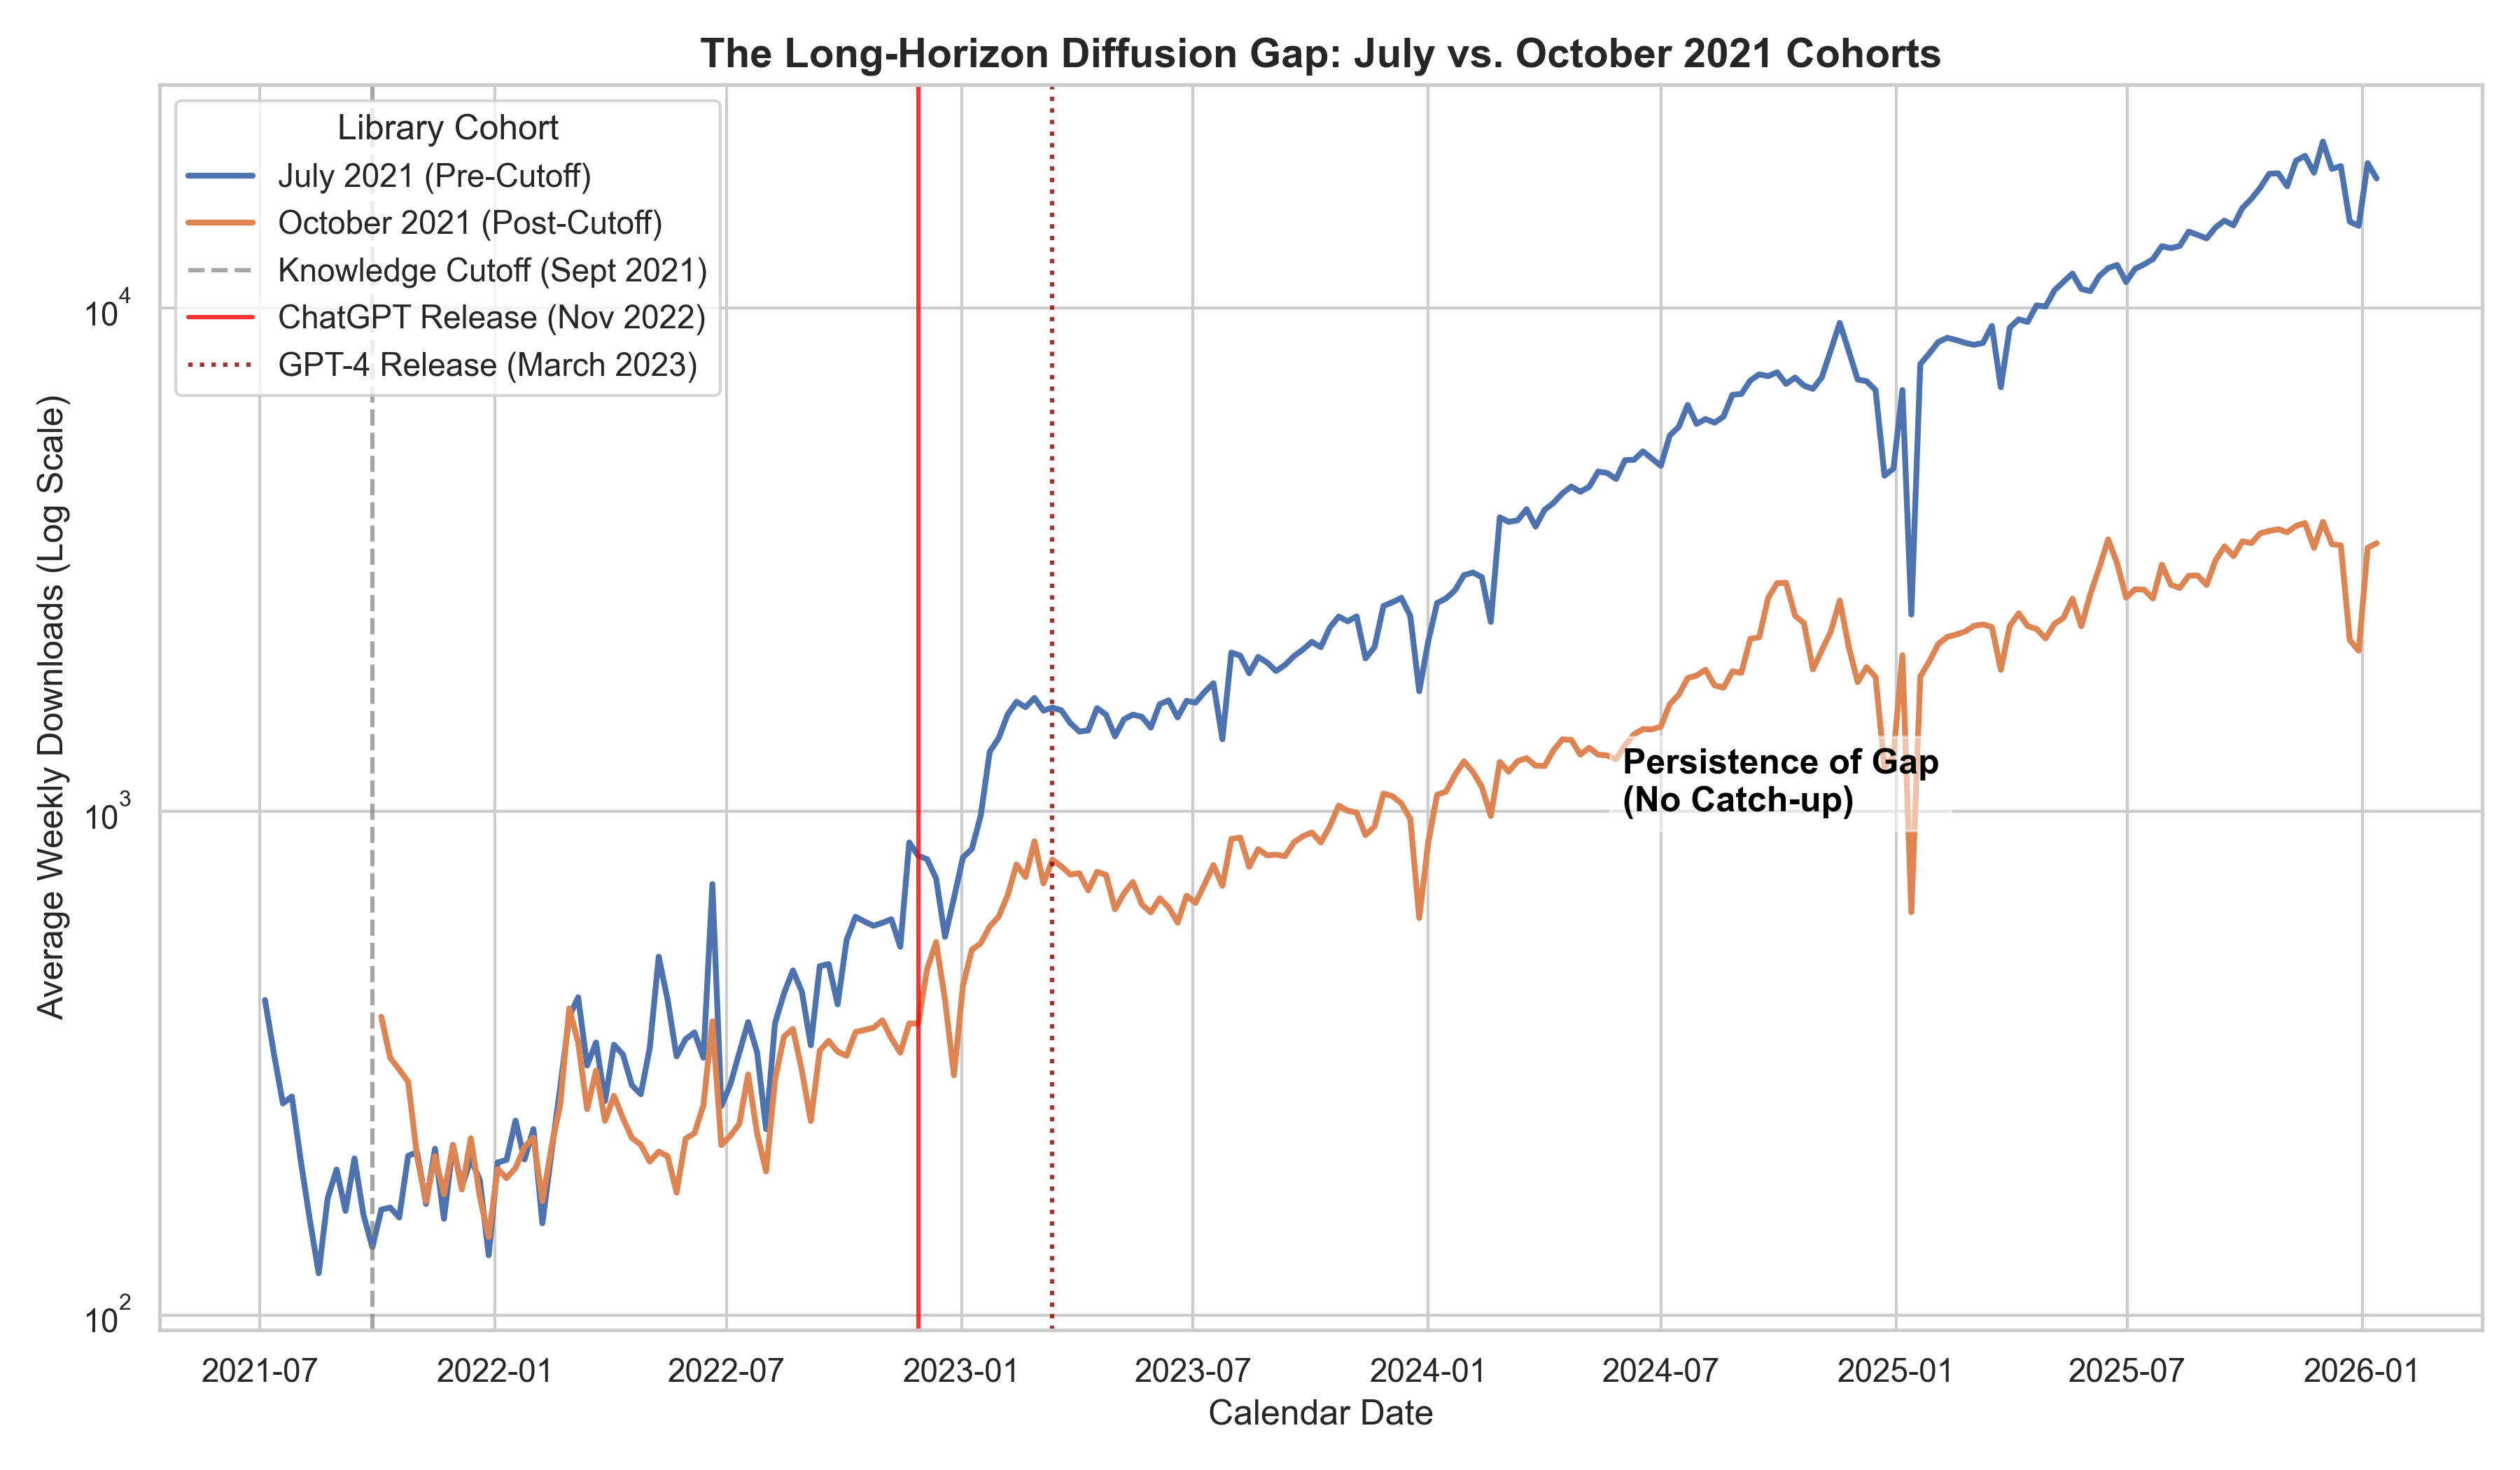
\includegraphics[width=0.85\textwidth]{results/figures/long_horizon_trajectory_pypi.png}
\caption{Weekly average PyPI downloads for the July 2021 (pre-cutoff) and October 2021 (post-cutoff) cohorts, from release through January 2026. Dashed vertical lines mark ChatGPT release (November 2022) and GPT-4 release (March 2023). The gap between cohorts opens after ChatGPT and persists through the end of the observation window, with no evidence of catch-up.}\label{fig:long-horizon}
\end{figure}

Figure~\ref{fig:long-horizon} provides the visual analogue to the activation hypothesis. The two cohorts track each other closely before November 2022, after which the pre-cutoff cohort diverges upward. As of January 2026, the gap shows no sign of closing.

The sample selection of the GitHub-matched subsample warrants careful attention, because it interacts with the interpretation of the implementation gap in a substantive way. Within the near-cutoff window (libraries released within 26 weeks of the September 2021 boundary, donut excluded), the GitHub-matched sample contains 1,804 pre-cutoff and 2,341 post-cutoff libraries. Among these, 86.8\% of pre-cutoff libraries and 92.0\% of post-cutoff libraries qualify as Successful (at least 500 pre-ChatGPT downloads), a 5.2 percentage point advantage for the post-cutoff group. The GitHub-matched post-cutoff sample is therefore more selected for demonstrated pre-AI quality than its pre-cutoff counterpart. This selection works against detecting a suppression effect: if post-cutoff libraries in the matched sample are disproportionately high-quality, their post-AI import disadvantage cannot be attributed to a quality difference between the groups. The suppression estimate derived from this sample is accordingly conservative.

The selection pattern is also visible in implementation survival rates. Among GitHub-matched Successful-tier libraries in the near-cutoff window, 44.1\% of pre-cutoff and 42.5\% of post-cutoff libraries accumulate at least 10 post-AI all-time imports; 14.3\% of pre-cutoff versus 12.6\% of post-cutoff libraries accumulate at least 100 imports. These raw differences are small in absolute terms and are not adjusted for running variable continuity. They are, however, directionally consistent with the RDD estimates: post-cutoff libraries are less likely to achieve implementation traction at every threshold, despite being more selected for pre-AI quality. The log-point RDD estimates (+26.8 for post-AI imports) capture the sharp local discontinuity at the boundary that these sample-average rates smooth over.

\section{Mechanism Moderation Test}\label{sec:results-moderation}
The formal test is an interacted WLS model estimating whether the discontinuity differs between High AI and Low AI libraries.

\begin{table}[h!]
\centering
\caption{AI Exposure Moderation (Exploratory)}\label{tab:mechanism}
\small
\begin{threeparttable}
\begin{tabular}{lcccc}
\toprule
\textbf{Outcome} & \textbf{Interaction ($\delta$)} & \textbf{SE} & \textbf{p-value} & \textbf{N} \\ \midrule
52-week Downloads & +0.396 & 0.295 & 0.179 & 1,303 \\
52-week Imports & +0.257 & 0.292 & 0.380 & 1,303 \\ \bottomrule
\end{tabular}
\begin{tablenotes}
\small
\item \textit{Notes:} Interacted WLS with week-clustered standard errors. Triangular kernel, $h = 26$ weeks, 9-week asymmetric donut. Bandwidth differs from the main Diff-in-RDD ($h = 13$) to retain sufficient observations for the split-sample design. High AI libraries are those above the median of \texttt{avg\_ai\_score\_52wk} in the GitHub-matched subsample.
\end{tablenotes}
\end{threeparttable}
\end{table}

Neither interaction is statistically significant. With $N = 1{,}303$ and approximately 650 observations per AI-exposure group, the interacted split-sample RDD is almost certainly underpowered to detect meaningful moderation. The null result should therefore be interpreted primarily as reflecting insufficient statistical power rather than as positive evidence for a systemic effect. The data cannot distinguish between a broad ecosystem-wide penalty and a targeted effect on AI-mediated usage that the test lacks the power to detect.

\section{Bandwidth Sensitivity and Robustness Checks}\label{sec:results-robustness}

\textbf{Bandwidth sensitivity.} Main Diff-in-RDD estimates are stable across $h \in \{13, 18, 26, 39\}$ weeks, in both sign and approximate magnitude. Results at $h = 10$ are imprecise due to the donut exclusion compressing the effective estimation sample and are excluded from the primary evidence base. Figure~\ref{fig:bw-sensitivity} displays the Diff-in-RDD excess jump across bandwidths.

The GitHub implementation estimates are not subject to a Diff-in-RDD counterpart and are more sensitive to bandwidth choice than the PyPI Diff-in-RDD. At $h = 13$ weeks the post-AI import discontinuity is 26.8 log points ($p = 0.014$); at $h = 18$ weeks it falls to 2.9 log points ($p = 0.129$). These estimates are therefore treated as descriptive evidence consistent with the channel interpretation, not as independently robustified causal estimates.

\begin{figure}[ht]
\centering
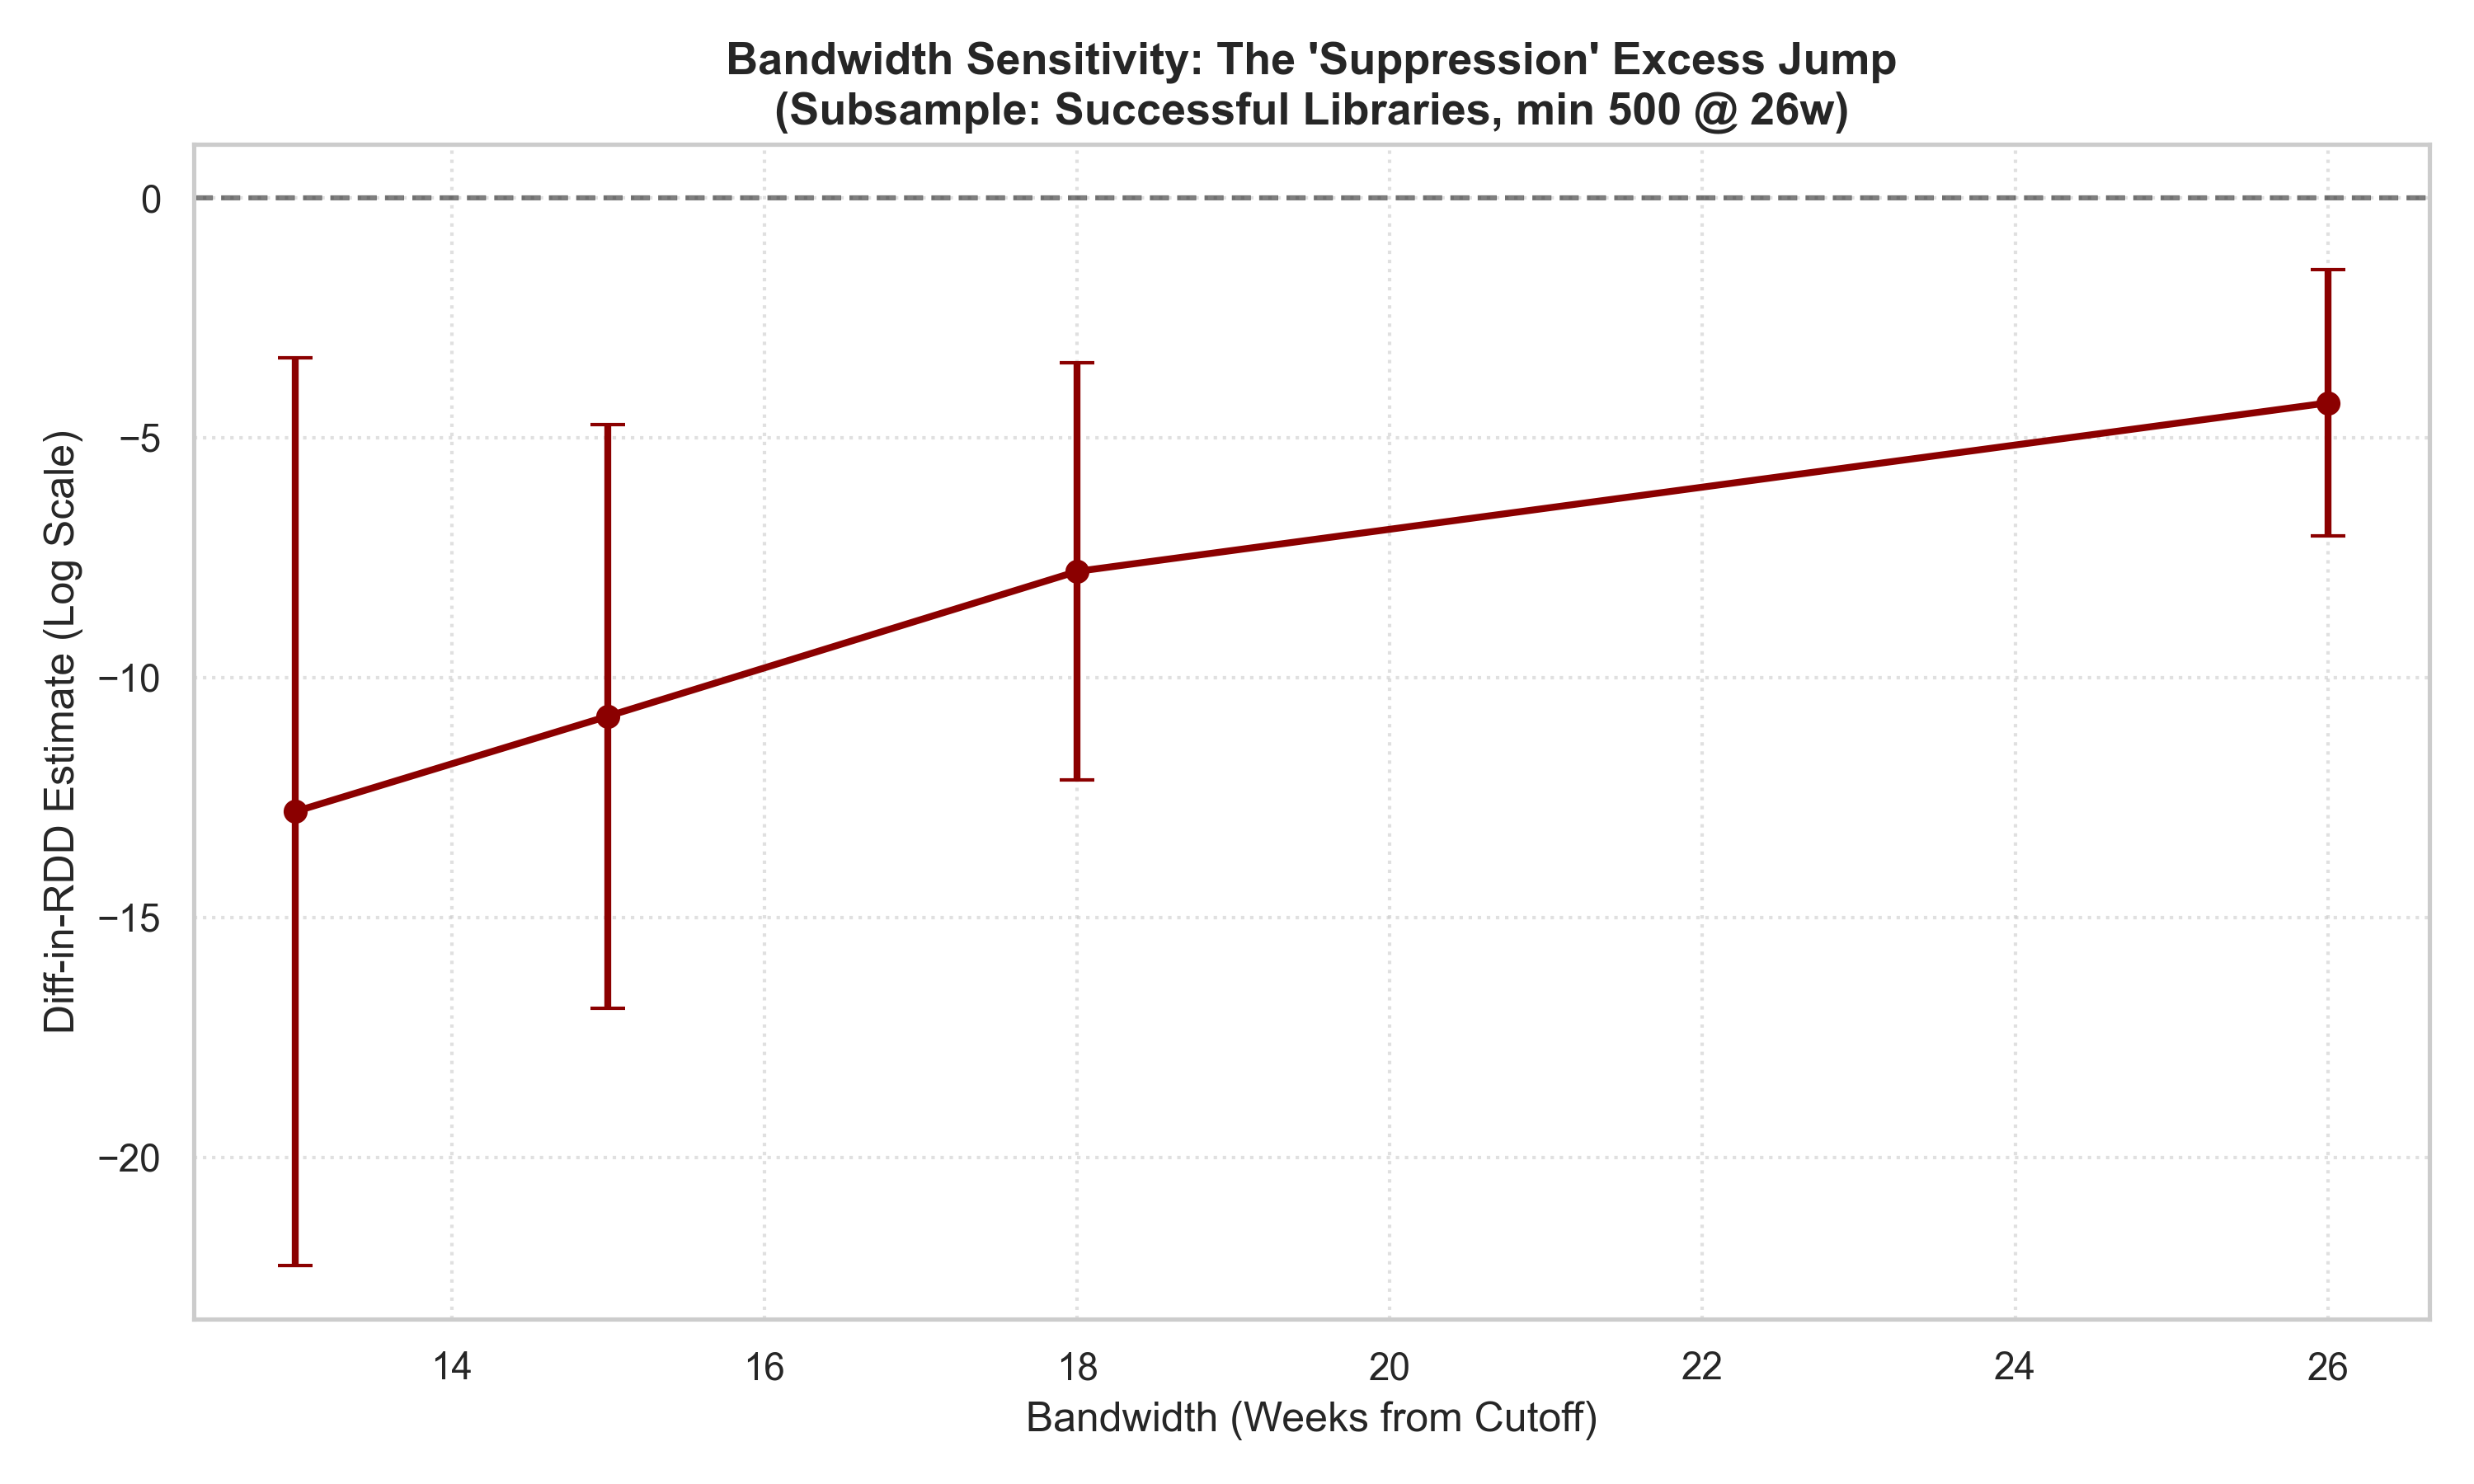
\includegraphics[width=0.85\textwidth]{results/figures/sensitivity_diff_in_rdd_bandwidth.png}
\caption{Bandwidth sensitivity of the Diff-in-RDD excess jump (Successful tier, min.\ 500 downloads at 26 weeks). Points are WLS point estimates; vertical bars are 95\% confidence intervals from year-by-week cluster-robust standard errors. The estimate is negative and stable across $h \ge 13$.}\label{fig:bw-sensitivity}
\end{figure}

\textbf{Symmetric donut.} Replacing the asymmetric 9-week donut with a symmetric $\pm 4$-week exclusion produces qualitatively consistent results. Quantitative differences across donut designs are modest and do not alter the direction or significance of the main findings.

\textbf{Density test.} No significant discontinuity in the density of release dates at the cutoff is detected by the McCrary test (see Figure~\ref{fig:density} in Chapter~\ref{ch:data}), providing no evidence for systematic sorting of releases around the September 2021 boundary.

\textbf{Permutation inference.} The moving-cutoff permutation test (Section~\ref{sec:methods-permutation}) yields a two-sided empirical $p$-value of 0.344 for the raw RDD estimate at the September 2021 cutoff. That is, the raw 52-week download discontinuity at the true cutoff is not statistically unusual relative to discontinuities observed at arbitrary placebo dates. Figure~\ref{fig:permutation} shows the distribution of placebo RDD coefficients with the true estimate marked.

\begin{figure}[ht]
\centering
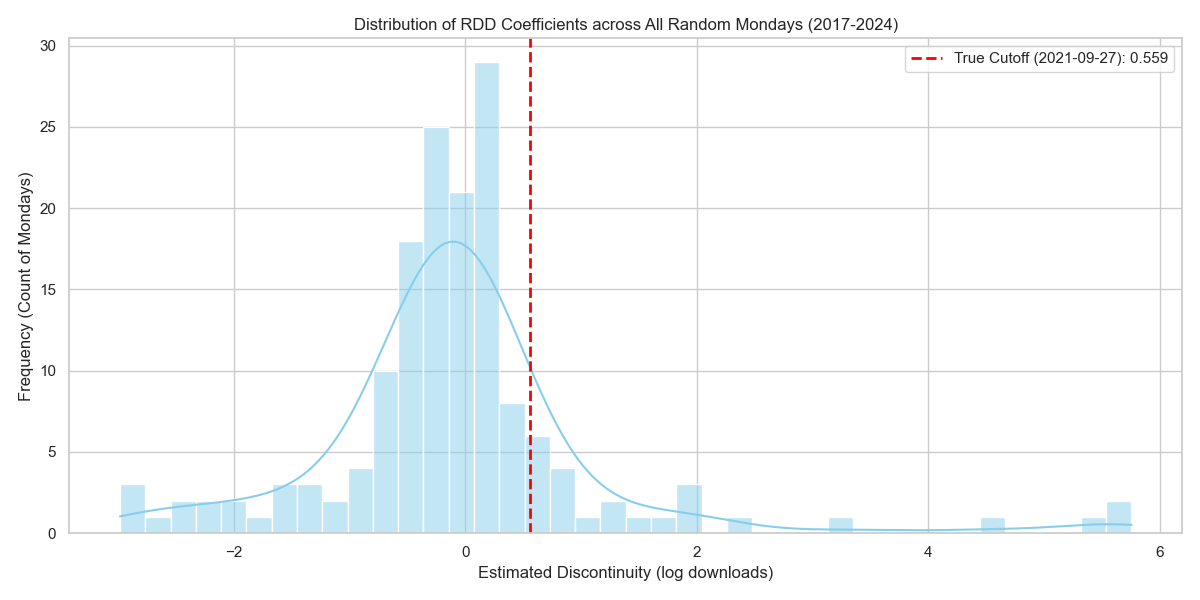
\includegraphics[width=0.85\textwidth]{results/figures/permutation_distribution.png}
\caption{Distribution of RDD coefficients across 157 placebo Monday cutoff dates (2017--2024). The dashed red line marks the true September 2021 cutoff estimate (+0.559 log points). The true estimate falls within the body of the placebo distribution ($p = 0.344$), confirming that the raw RDD is not informative in isolation.}\label{fig:permutation}
\end{figure}

This result is expected: the raw RDD captures a composite of the Knowledge Wall effect and a seasonal pattern common to all September release windows. The permutation test cannot isolate the cutoff-specific component, which is precisely why the Diff-in-RDD, not the raw RDD, serves as the primary causal specification. The non-significance of the raw permutation test reinforces the identification argument for the Diff-in-RDD design.

% ------------------------------------------------------------------
% Chapter 6
% ------------------------------------------------------------------
\chapter{Discussion}\label{ch:discussion}

\section{What the Evidence Shows}\label{sec:disc-evidence}
The research question is whether Python libraries released shortly before the GPT-3.5/GPT-4 training cutoff diffuse more widely in the AI era than libraries released shortly after, because the former are more likely to be represented in the model's pretrained knowledge. The evidence supports an affirmative answer with high confidence in the main finding and qualified confidence in the mechanism.

The core result, a $-12.8$ log point penalty in post-AI cumulative downloads for Successful post-cutoff libraries (Diff-in-RDD, $p = 0.008$), survives placebo testing, is robust across bandwidths, and is amplified in the outcome most directly attributable to LLM-generated code (GitHub imports, $+26.8$ log points). The absence of any comparable discontinuity in the 2018--2020 placebo cohorts and the activation pattern (the gap emerging only after November 2022 when LLMs became a mass interface) are consistent with the proposed mechanism.

\section{The Knowledge Wall: Framing and Interpretation}\label{sec:disc-wall}
The findings are organized around the concept of a \textbf{Knowledge Wall}: a structural discontinuity in the information landscape of deployed LLMs, created by the hard temporal boundary of their training data. Libraries on the pre-cutoff side of the wall are represented in the model's parametric knowledge and are therefore candidates for recommendation, code generation, and documentation synthesis. Libraries on the post-cutoff side are invisible to this channel.

This framing has three implications:
\begin{enumerate}
    \item The Knowledge Wall is an architectural property of static-knowledge models, operating regardless of developer awareness.
    \item The wall is asymmetric; pre-cutoff libraries benefit from the absence of a barrier that post-cutoff libraries face.
    \item The effects are expected to be persistent. As of early 2026, no catch-up is observed (Figure~\ref{fig:cumulative-gap}). The all-time implementation gap (+27.9 log points) suggests the divergence has accumulated rather than narrowed.
\end{enumerate}

The absence of a significant effect for the Superstar tier (at least 1,000 pre-ChatGPT downloads, $p = 0.261$) is consistent with this framing. Libraries that achieved the highest early visibility before ChatGPT are more likely to have accumulated organic adoption through channels largely independent of LLM recommendation: conference presentations, influential blog posts, direct dependency chains, and word-of-mouth within specialist communities. The Knowledge Wall operates most forcefully at the margin of entry, where LLM-mediated discovery is most consequential; it does not appear to override momentum already built through high-visibility human adoption.

\begin{figure}[ht]
\centering
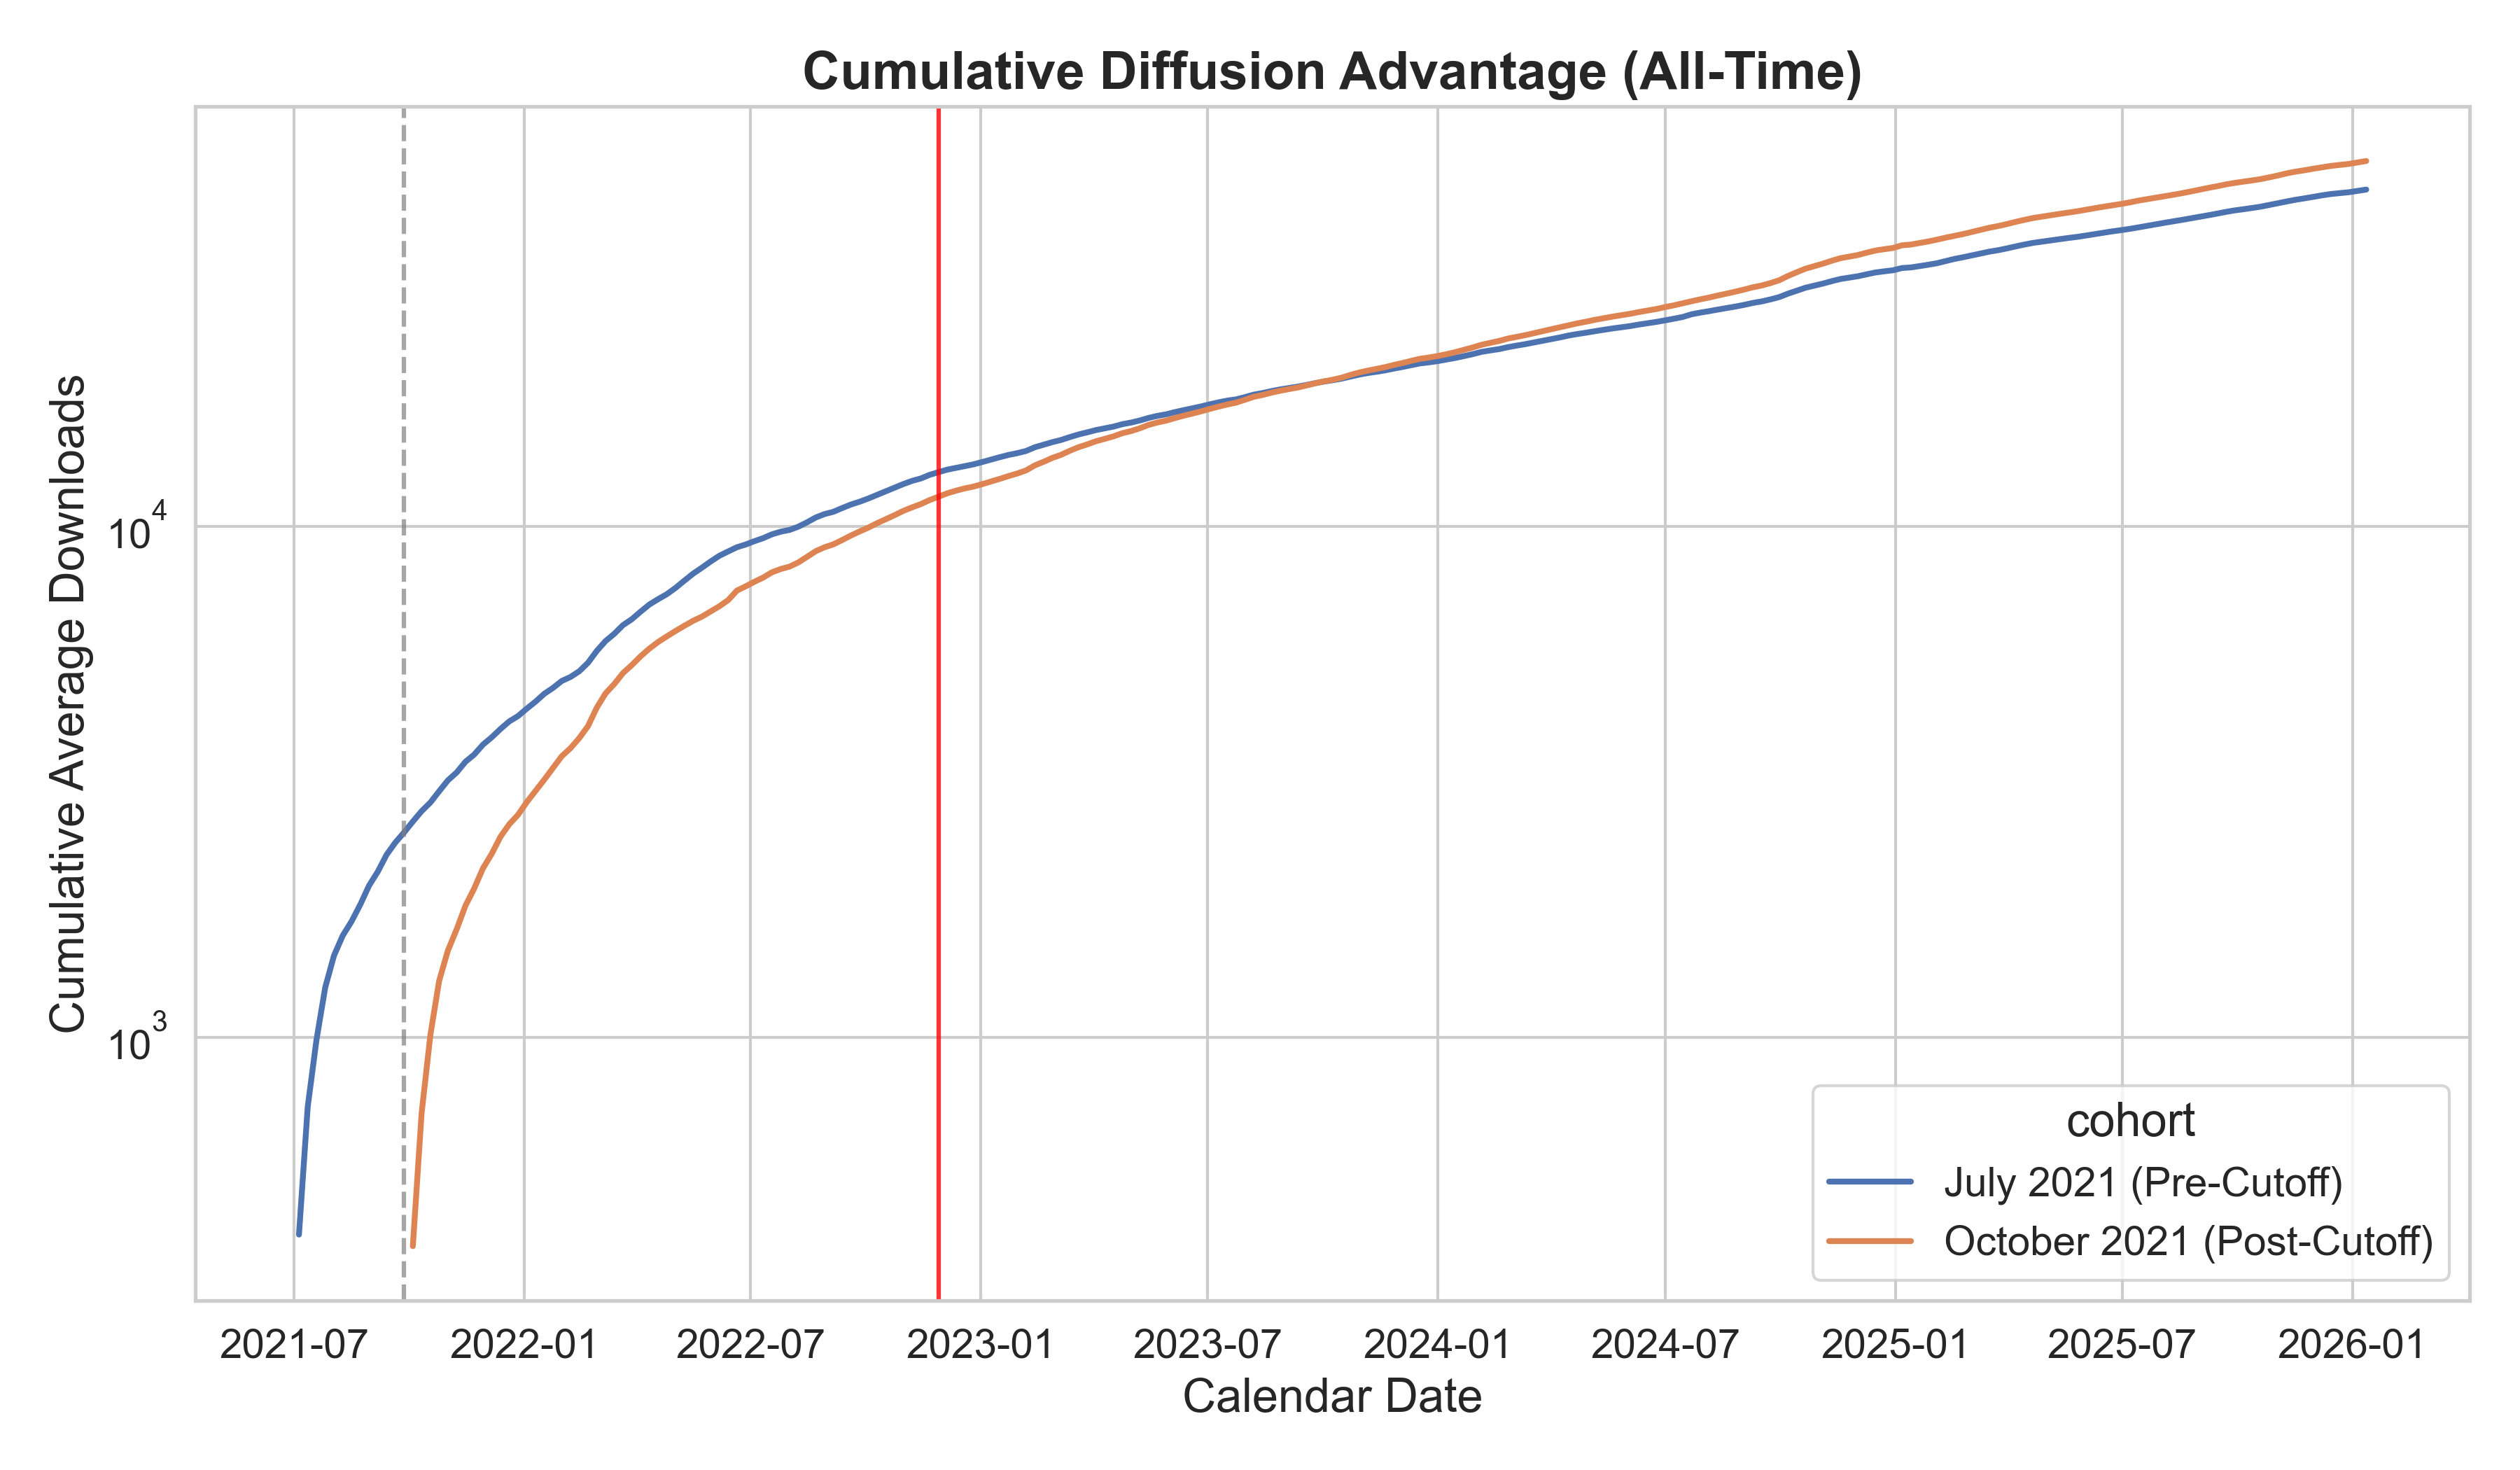
\includegraphics[width=0.85\textwidth]{results/figures/long_horizon_cumulative_pypi.png}
\caption{Cumulative average PyPI downloads for the July 2021 (pre-cutoff) and October 2021 (post-cutoff) cohorts. The vertical red line marks ChatGPT release (November 2022). The gap between cohorts widens monotonically after November 2022, with no catch-up through January 2026.}\label{fig:cumulative-gap}
\end{figure}

\section{Connection to \citet{doshi2024generative}}\label{sec:disc-doshi}
The conceptual foundation draws on \citet{doshi2024generative}, who demonstrate that generative AI improves individual creative quality while reducing collective diversity through convergence. The parallel to this paper is structural: AI steers developers toward convergent tool choices — specifically, tools established before the knowledge cutoff. Individual developers gain productivity (individual enhancement), but the aggregate effect is a concentration of adoption around the pre-cutoff library set (collective narrowing).

\section{Alternative Mechanisms and Threats to Interpretation}\label{sec:disc-threats}
The most immediate alternative explanation for a discontinuity at September 2021 is \textbf{calendar seasonality}: post-summer releases entering a high-activity development period. This is exactly what the Diff-in-RDD removes. The placebo cohorts (2018--2020) provide an estimate of the typical September discontinuity; the 2021 excess is residual after that baseline is subtracted. The significance of the excess jump ($p = 0.008$ for the Successful tier) is therefore not attributable to seasonal patterns.

A more subtle threat is \textbf{quality sorting}: libraries released just before and just after the cutoff may differ systematically in quality. The success tier logic addresses this directly. The Successful tier requires at least 500 downloads within 26 weeks, measured entirely before November 2022. Conditioning on this tier ensures a comparison of libraries that demonstrated comparable human-evaluated quality in the pre-AI period. The continued significance of the excess jump in this subsample is therefore difficult to attribute to quality sorting.

An important source of imprecision is the \textbf{exact location of the training cutoff within September 2021}. OpenAI's documentation states that the GPT-3.5 and GPT-4 training data ends in ``September 2021'' without specifying a day. The cutoff date used in this paper (September 27, the last Monday of the month) is a researcher choice, not an institutionally documented boundary. The true cutoff could be September 1, September 15, or any date within the month. This ambiguity is the primary motivation for the 9-week asymmetric donut, which excludes all libraries released in August and September 2021 from the estimation sample. Libraries in this window have genuinely uncertain training inclusion status, and removing them ensures that the comparison is between libraries clearly before the cutoff (July and earlier) and libraries clearly after it (October and later). The estimates are therefore robust to any cutoff placement within September, at the cost of reduced effective sample size near the boundary. More broadly, the running variable (weeks relative to a date that is not precisely documented) has non-classical measurement error. In the RDD context, measurement error in the running variable biases estimates toward zero, making the reported effects conservative.

A related concern is \textbf{GitHub Copilot as a near-simultaneous confounder}. Copilot was released in public preview in June 2021, three months before the September 2021 cutoff, and its underlying Codex model was trained on a corpus with a similar temporal boundary. Because Copilot and the GPT-3.5/GPT-4 family share an approximately overlapping knowledge cutoff, the estimated suppression cannot be attributed to a single model. Rather, the September 2021 boundary represents a shared knowledge cutoff across the dominant LLM-based coding tools deployed in 2022--2023. The causal claim is therefore best understood as the effect of the \textit{knowledge boundary as a class}, the date at which the major deployed LLMs stopped ingesting new training data, rather than the effect of any one product. This does not weaken the finding: it implies that the Knowledge Wall is a property of the model ecosystem's shared training infrastructure, not an idiosyncratic feature of ChatGPT alone.

\textbf{General platform dynamics} offer an alternative to the LLM-specific story: any technology platform that directs developer attention could in principle produce comparable discontinuities. If the suppression were driven by a general attention platform, however, there is no reason to expect GitHub implementation (code imports) to be more affected than PyPI downloads. The roughly 2:1 ratio of the discontinuity in GitHub versus PyPI is consistent with the LLM code generation channel specifically, not general attention dynamics.

Finally, \textbf{retrieval-augmented generation (RAG) and web search} capabilities in modern LLMs could in principle erode the knowledge asymmetry: a model that can retrieve current documentation at query time is no longer bounded by its training cutoff. Several considerations limit this objection. First, the timeline is inconsistent with real-time retrieval as an active mitigant during the critical mass-deployment window. ChatGPT launched in November 2022 without web access; the optional Browsing plugin was not available until March 2023 and required explicit user activation. GitHub Copilot, the dominant code completion tool, does not retrieve external documentation by default. The period in which the Knowledge Wall would have had its largest marginal effect on newly released libraries (late 2022 through 2023) therefore substantially predates widespread retrieval availability. Second, even where retrieval is technically available, its practical adoption for routine coding tasks is limited. \citet{gao2024retrieval} document persistent limitations in deployed RAG systems: retrieval quality is unreliable for technical queries, latency costs are substantially higher than parametric inference, and accuracy degrades with longer retrieved contexts due to attention dilution. For the dominant use case examined here (a developer asking an LLM to suggest or implement a library for a task) parametric knowledge remains the default path, as retrieval would require the model to discover and index the target library before it could recommend it. Third, the empirical trajectory is inconsistent with retrieval as an active corrective. If real-time retrieval were eroding the Knowledge Wall, the implementation gap should narrow or close as web-enabled models become standard. Figure~\ref{fig:long-horizon} shows the opposite: the gap widens through early 2026. This pattern is more consistent with parametric knowledge remaining the operative channel in production deployments than with retrieval progressively restoring access to post-cutoff libraries.

\section{The Systemic Wall Interpretation}\label{sec:disc-systemic}
The mechanism moderation test found no significant heterogeneity between High and Low AI exposure libraries ($p = 0.179$). This suggests the Knowledge Wall operates as a broad ecosystem effect. LLMs serve as a general discovery and documentation interface; exclusion from this interface reduces discoverability across the entire software stack, not just in AI-heavy contexts.

\section{Scope Conditions and External Validity}\label{sec:disc-scope}
The estimated effect is a Local Average Treatment Effect at the September 2021 cutoff boundary. It identifies the expected difference in diffusion for a library released just after the cutoff relative to one released just before. This is not necessarily the effect for libraries released far from the cutoff; for example, a library released three years post-cutoff, which has had time to accumulate community adoption through other channels. The local estimate is the most defensible claim; extrapolation to the full ecosystem is speculative.

The design exploits one documented cutoff date. Different cutoffs (for Claude, Gemini, Llama, and subsequent GPT versions) would produce overlapping exclusion windows that are harder to isolate. Whether the findings generalize to other cutoff dates is an open empirical question that would require a multi-cutoff design.

Python is a particularly LLM-influenced ecosystem: it is the dominant language for data science and machine learning, where AI-assisted coding is most prevalent. The effect size identified here may be larger than what would be found in languages or ecosystems with less AI-mediated developer activity. Replication in other language ecosystems (e.g., npm for JavaScript, crates.io for Rust) would establish whether the Knowledge Wall is a general phenomenon or specific to the AI-adjacent Python community.

The analysis focuses on libraries in their first weeks and months of existence. Established libraries with large existing user bases are less susceptible to the Knowledge Wall because they achieve diffusion through mechanisms independent of LLM recommendation: direct network effects, conference presentations, existing dependency chains. The effect is expected to be largest at the emergence stage, where new libraries depend most heavily on discovery mechanisms.

\section{Limitations}\label{sec:disc-limitations}
Key limitations include running variable measurement error (PyPI registration lags), matching coverage (the 5.3\% GitHub match rate over-represents prominent libraries), and the endogeneity of the AI exposure moderator. The causal claim rests on the parallel trends assumption for the Diff-in-RDD, which is supported by placebo stability but remains fundamentally untestable.

\textbf{Multiple testing.} The paper reports RDD estimates across multiple outcomes (52-week downloads, post-AI downloads, several GitHub import horizons), three success tiers, and two designs (main RDD and Diff-in-RDD). No family-wise error correction (e.g., Bonferroni or Benjamini--Hochberg) is applied. The probability of observing at least one significant result by chance across this many tests is non-trivial. The primary defense is that the results are not cherry-picked from a large search: the Diff-in-RDD for the Successful tier ($p = 0.008$) is designated as the main specification \textit{ex ante}, the activation pattern is consistent across horizons, and the direction of effects is stable across tiers. Nonetheless, readers should interpret marginal results (e.g., the Broad-tier Diff-in-RDD at $p = 0.039$) with additional caution.

\textbf{Secular growth in the Python ecosystem.} The Diff-in-RDD assumes that the seasonal pattern at the September boundary is stable across 2018--2021. If the Python ecosystem experienced accelerating growth over this period, with each successive year producing more downloads per library than the last, the 2018--2020 placebo baseline would understate the expected 2021 seasonal jump, biasing the excess jump estimate away from zero. The placebo cohorts do not show a monotonic trend in their individual discontinuity estimates, which provides some reassurance, but a formal test for trend in placebo discontinuities has not been conducted. This threat cannot be fully ruled out.

\section{Implications}\label{sec:disc-implications}
\textbf{For library authors:} Release timing relative to major LLM cutoffs is a determinant of adoption probability. Post-cutoff releases face a structural disadvantage that quality alone may not offset.

\textbf{For the software ecosystem:} If LLMs function as concentration mechanisms, successive model generations may reinforce existing adoption hierarchies, potentially slowing the turnover of the dominant tool set and stifling innovation at the frontier.

% ------------------------------------------------------------------
% Chapter 7
% ------------------------------------------------------------------
\chapter{Conclusion}\label{ch:conclusion}

This paper asked whether the training-data cutoff of large language models affects the diffusion of newly released open-source software. Exploiting the September 2021 knowledge boundary shared by the GPT-3.5 and GPT-4 model families, I estimated a regression discontinuity in the adoption trajectories of Python libraries released just before versus just after the cutoff, using PyPI download counts and GitHub import data. A Difference-in-Discontinuities design, which differences the 2021 discontinuity against placebo discontinuities at the same calendar position in 2018--2020, provides the primary causal estimate.

The answer to the research question is affirmative. Libraries released just after the cutoff, excluded from the dominant LLMs' parametric knowledge, accumulate significantly fewer downloads and code imports once those models reach mass deployment. The Diff-in-RDD estimate for libraries that demonstrated pre-AI quality (at least 500 downloads within 26 weeks, measured entirely before ChatGPT) is $-12.8$ log points ($p = 0.008$). The suppression is approximately twice as large in GitHub code imports as in aggregate PyPI downloads, consistent with LLM-steered code generation as the operative channel. Three placebo cohorts show no comparable discontinuity, and the gap activated only after November 2022, when ChatGPT provided a mass interface through which the training boundary became consequential. As of January 2026, no catch-up is observed. The suppression is concentrated in the Broad and Successful tiers; libraries with the highest pre-ChatGPT visibility (Superstar tier, at least 1,000 downloads) show no significant penalty ($p = 0.261$), consistent with very high-visibility libraries maintaining adoption through channels independent of LLM recommendation.

These findings support the existence of what this paper terms a Knowledge Wall: a structural barrier created by the hard temporal boundary of LLM training data. The wall redirects early adoption toward libraries already represented in the model's knowledge, penalizing post-cutoff entrants regardless of their quality. The mechanism is consistent with the broader theoretical concern, articulated by \citet{doshi2024generative} in the context of creative output, that generative AI may enhance individual capability while narrowing collective variety. In the software ecosystem, the variety that narrows is the set of tools in active use; the individual enhancement is the productivity gain from AI-assisted coding; and the structural cause is the fixed knowledge boundary that determines which tools the AI can recommend.

This paper makes three contributions. First, it provides a quasi-experimental estimate of the causal effect of an LLM training boundary on software adoption, exploiting a precisely dated institutional feature for identification. Second, it introduces a two-outcome design (PyPI downloads versus GitHub imports) that isolates the code generation channel from general discoverability. Third, it demonstrates that a pre-AI quality advantage for post-cutoff libraries (28.6 percentage points more likely to reach the Successful tier before ChatGPT) reverses into a post-AI deficit, establishing that the suppression cannot be attributed to pre-existing differences in library quality.

Several limitations bound the conclusions. The running variable is constructed from first observed download dates, a noisy proxy for true release timing that biases estimates conservatively. The training cutoff date itself is documented only at the month level; the specific day (September 27) is a researcher assignment, and the asymmetric donut exclusion is the primary defense against this ambiguity. The GitHub-matched subsample covers 5.3\% of the PyPI universe and over-represents prominent libraries, limiting the external validity of the implementation gap estimates. The exploratory mechanism test (whether suppression is stronger among libraries with higher AI-exposure scores) is non-significant ($p = 0.179$), but the moderator is post-treatment and the test is underpowered ($N = 1{,}303$), so the null cannot distinguish a broad ecosystem effect from an undetectable targeted one. Finally, the estimates are local to a narrow window around a single cutoff date and should not be extrapolated to the full ecosystem or to distant time horizons without further evidence.

Several questions remain open. First, as model providers adopt more frequent retraining schedules and retrieval-augmented generation becomes standard, the knowledge asymmetry may diminish. Whether the Knowledge Wall is a transitional feature of the current generation of static-knowledge models or a durable property of AI-mediated ecosystems is an empirical question that can only be answered longitudinally. Second, replication at other cutoff dates (for Claude, Gemini, Llama, and subsequent GPT versions) would establish whether the finding generalizes beyond the September 2021 boundary. Third, replication in other language ecosystems (npm, crates.io, CRAN) would test whether the effect is specific to Python's AI-adjacent developer community or a general feature of LLM-mediated software adoption. Fourth, the mechanism test deserves a dedicated design: a larger matched sample with an exogenous measure of AI exposure could determine whether the wall operates through code generation specifically or through a broader shift in developer information acquisition. Finally, the welfare implications of the Knowledge Wall (whether the redirection of adoption toward pre-cutoff tools is costly or merely redistributive) depend on the substitutability of pre- and post-cutoff libraries, a question this paper does not address.

The broader implication is that LLMs, by fixing a temporal boundary in their training data and mediating an increasing share of developer decision-making, have introduced a new structural determinant of technology adoption. The Knowledge Wall is not the result of deliberate gatekeeping or market power; it is an architectural byproduct of how these models are built. Its consequences, however, are distributional: they fall on the developers and projects that happen to arrive after the boundary. Understanding and mitigating this asymmetry is a design problem for the next generation of AI-assisted development tools.

% ------------------------------------------------------------------
% Bibliography
% ------------------------------------------------------------------
\bibliographystyle{apalike}
\bibliography{references}

% ------------------------------------------------------------------
% Appendix
% ------------------------------------------------------------------
\appendix

\chapter{Declaration of AI Tool Usage}\label{app:ai-declaration}

In accordance with the BCE TDK competition rules (Section IV.1.b), the following declaration describes all uses of artificial intelligence tools during the preparation of this paper. Three AI tools were used, each restricted to minor subtasks as defined by the competition rules.

\section*{Tools Used}

\begin{enumerate}
    \item \textbf{Claude (Anthropic, Claude Code CLI).} Used for literature search and orientation (identifying potentially relevant papers for manual verification), language and grammar checking of English-language prose, and LaTeX formatting assistance (table layout, equation typesetting, document structure).
    \item \textbf{Gemini CLI (Google).} Used for brainstorming research design alternatives, exploring the structure of robustness checks, and debugging Python scripts during data pipeline development.
    \item \textbf{GitHub Copilot (Microsoft).} Used for code autocompletion during the development of data processing and estimation scripts in Python.
\end{enumerate}

\section*{Research Process}

During the research process, Claude and Gemini were used interactively to explore ideas, outline arguments, and produce preliminary drafts that served as working material. The final text was written by the author. All empirical results were produced by the author's own code executing established statistical packages (\texttt{rdrobust}, \texttt{statsmodels}, \texttt{pandas}). The research question, identification strategy, variable definitions, specification choices, and interpretation of findings are the author's own work, developed in consultation with the supervisor. No AI tool autonomously generated empirical results, made research design decisions, or produced text that appears in the submitted version without having been rewritten by the author.

\end{document}